\documentclass[final]{llncs}
\usepackage{llncsdoc}
\usepackage{fainekos-macros}
\usepackage{color}


\usepackage[english]{babel}
\usepackage{amsmath}
\usepackage{graphicx}
\usepackage[colorinlistoftodos,obeyFinal]{todonotes}
\usepackage{wrapfig}
\usepackage{makeidx}  % allows for indexgeneration
\usepackage{bibspacing}
\usepackage{fancyvrb}
\usepackage{amsfonts}
\usepackage{color}
\usepackage[ruled]{algorithm}
\usepackage{algpseudocode}
\usepackage{authblk}

\setlength{\bibspacing}{\baselineskip}
\usepackage[tight,footnotesize]{subfigure}

\newcommand{\mySection}[1]{\vspace{-5pt}\section{\hskip -1em.~~#1}\vspace{-10pt}}
\newcommand{\mySubSection}[1]{\vspace{-5pt}\subsection{\hskip -1em.~~#1}\vspace{-10pt}}
\newcommand{\mySubSubSection}[1]{\vspace{-5pt}\subsubsection{\hskip -1em.~~#1}\vspace{-5pt}}
\newcommand{\tableref}[1]{Table~\ref{tab:#1}}
\newcommand{\figref}[1]{Fig.~\ref{fig:#1}}
\newcommand{\Hao}[1]{$\clubsuit$\footnote{HAO: #1}}
\newcommand{\hatodo}[1]{\todo{HA: #1}}
\newcommand{\hatodoin}[1]{\todo[inline]{HA: #1}}
\newboolean{TECH_REPORT}
\newcommand{\beh}{\mathbb{B}}
\newcommand{\straj}{\mathbf{x}}
\newcommand{\absfun}{h}
\DeclareSymbolFont{extraup}{U}{zavm}{m}{n}
\DeclareMathSymbol{\varheart}{\mathalpha}{extraup}{86}
\DeclareMathSymbol{\vardiamond}{\mathalpha}{extraup}{87}
\setlength{\textwidth}{12.5cm}
\setlength{\textheight}{20.4cm}
%\setlength{\oddsidemargin}{-.204in}

\setboolean{TECH_REPORT}{TRUE}

\title{Abstraction Trees for Closed-Loop Model Checking of Medical Devices\thanks{This work was supported by NSF CAREER 1253842, NSF MRI 1450342 and STARnet, a Semiconductor Research Corporation program, sponsored by MARCO and DARPA.}}

\author{Zhihao Jiang\inst{1} \and Houssam Abbas\inst{1},
Pieter J. Mosterman\inst{2,}\inst{3} \and Rahul Mangharam\inst{1}}
\institute{Department of Electrical and Systems Engineering, University of Pennsylvania
\and
School of Computer Science, McGill University, Canada \and MathWorks, USA}

\begin{document}
\maketitle
\vspace{-15pt}
\begin{abstract}
Ventricular Fibrillation is a disorganized electrical excitation of the heart that results in inadequate blood flow to the body.
It usually ends in death within seconds.
The most common way to treat the symptoms of fibrillation is to implant a medical device, known as an \emph{Implantable Cardioverter Defibrillator} (ICD), in the patient's body.
Model-based verification can supply rigorous proofs of safety and efficacy. 
In this paper, we build a hybrid system model of the human heart+ICD closed loop, and show it to be a \yhl{STORMED system, a class of o-minimal hybrid systems that admit finite bisimulations.}
In general, it may not be possible to compute the bisimulation.
We show that approximate reachability can yield a finite \emph{simulation} for STORMED systems, which improves on the existing verification procedure.
In the process, we show that certain compositions respect the STORMED property.
Thus it is possible to model check important formal properties of ICDs in a closed loop with the heart, such as delayed therapy, missed therapy, or inappropriately administered therapy. 
The results of this paper are theoretical \yhl{and motivate the creation of concrete model checking procedures for STORMED systems.}
\end{abstract}

%Ventricular Fibrillation is a disorganized electrical excitation of the heart that results in inadequate blood flow to the body.
%It usually ends in death within a few seconds.
%The most common way to treat the symptoms of fibrillation is to implant a medical device, known as an Implantable Cardioverter Defibrillator (ICD), in the patient's body.
%Model-based verification can play a crucial role in ICD development.
%In this paper, we build a hybrid system model of the human heart+ICD closed-loop system, and show that it admits a finite bisimulation by showing it to be a STORMED hybrid system.
%In general, it may not be possible to compute the bisimulation.
%We show that approximate reachability can yield a finite \emph{simulation} for STORMED systems, which improves on the existing verification procedure.
%In the process, we show that certain compositions respect the STORMED property.
%Thus it is possible to model check important formal properties of ICDs in a closed loop with the heart, such as delayed therapy, missed therapy, or inappropriately administered therapy. 
%The results of this paper are theoretical, since no model checkers exist for STORMED systems. 
%In future work we will implement a procedure for model checking the heart+ICD loop.

\section{Introduction}
\label{introduction}

%\todo[inline]{stress the timing aspect more}
Implantable medical devices such as pacemakers are designed to improve physiological conditions with very little human intervention. 
Their ability to autonomously affect the physiological state of the patient makes the medical devices safety-critical, and sufficient evidence for their safety and efficacy should be provided before the devices can be implanted in the patients. Medical devices increasingly rely on software, and device function and their clinical performance can be affected by seemingly minor changes to software.
%As more functionality is added to the devices
\footnote{In what follows, the word `device' is used to refer to the software of the device.}
%, the complexity of the software component of the device is increasing dramatically, leading to a large number of potential safety violations because of software bugs. 

Over the course of the past four decades, cardiac rhythm management devices such as pacemakers and implantable cardioverter defibrillators (ICD) have grown in complexity and now have more than 80,000 to 100,000 lines of software code~\cite{pauljones}. In 1996, 10\% of \emph{all} medical device recalls were caused by software-related issues and this rose to 15\% between 2003-2012~\cite{recall_stats,killedbycode}. There is currently no standard for testing, validating, and verifying the software for implantable medical devices~\cite{fda1,fda3}.

There are two categories of device bugs: 
1) the device may fail to conform to its \emph{specifications}, that is, the prescription of how it should react to certain inputs.  
2) the device may fail to improve the conditions of the patient as promised, even if it conforms to its specifications. 
The desired physiological conditions that the closed-loop system should achieve are captured in the \emph{physiological requirements}; for example, for a pacemaker, the heart rate should always be maintained above a certain threshold. 
%In what follows, the word `requirement' always refers to such physiological requirements.
%Note that requirements are about \emph{the closed-loop system}: they prescribe the behavior of both device and environment (e.g. both pacemaker and heart).

Bugs in the first category (non-conformance to specification) can be detected via systematic and extensive open-loop testing in which a set of input sequences is fed to the device, and its output is compared with the expected output.
Bugs in the second category (violation of physiological requirements), on the other hand, require the availability of the \emph{closed-loop system}, which consists of the device and its environment.
For instance, the pacemaker and the heart as its environment. 
In the medical device industry, closed-loop verification of the physiological requirements is mostly performed in terms of clinical trials, in which the actual devices are implanted in human subjects over an extended duration.
Unfortunately, because of the extremely high cost of clinical trials (several million dollars and spanning several years~\cite{trial_cost}), the amount and variety of human subjects during the clinical trials are limited, which reduces the opportunity to find bugs. 
Moreover, clinical trials are often conducted at the final design stage. Fixing bugs at this stage is very costly.

Closed-loop model checking enables closed-loop evaluation of the physiological requirements at an earlier design stage, which requires formal model(s) of the physiological environment. 
%Depending on the formalism used to model the environment (and device) and the language used to express the requirements, this allows the usage of formal methods to perform the verification.
%Formal environment modeling introduces new challenges that do not arise when modeling the device alone, and this paper aims at addressing these issues in the context of pacemaker verification.
%In the rest of this paper, we speak therefore of pacemaker as the Device Under Verification (DUV) and of the heart as being the environment, but it is understood that the discussion carries more broadly, with possible domain-specific adjustments.
In closed-loop model checking, there is only one device model. 
However there can be a large number of environmental conditions which require different models to represent them. For instance, a heart with atrial flutter has an additional conduction pathway that is not present in a healthy heart, causing fast atrial rate. The timing and structural differences of different heart conditions should be distinguished in corresponding heart models.
%\todo[inline]{should we give an example of a heart condition?}
A set of initial models of the environment can be constructed but the set is inherently incomplete because of the large number of environment conditions and their combinations. 
As a result, performing model checking using every model in the set cannot ensure full coverage of the environmental conditions. 

In this paper, domain-specific over-approximation rules are developed that produce abstract models that not only cover explicitly modeled environment conditions, but also cover timing behaviors and conditions not modeled in the set of initial models. 
The abstract models can be then used for closed-loop model checking of the device model. 
If the closed-loop system satisfies a requirement, the device under verification satisfies the requirement under environment conditions covered by the abstract models. 
However, if the requirement is not satisfied, the model checker returns a counter-example. 
In device modeling, the counter-example is considered \emph{spurious} if it can not be produced by the device (as shown in (\figref{distinction}(a)).
However in environment modeling, even if the counter-example can not be produced by any of the initial environment models, it might still be a physiologically valid behavior.
Thus the validity of a counter-example cannot be determined by refining the environment model, but can ultimately only be determined by domain experts. 

Counter-examples returned from abstract models can be difficult to interpret by domain experts.
One abstract counter-example could be produced by multiple physiologically valid conditions, which causes ambiguity.
Thus, a rigorous framework is necessary to balance the need to cover a wide range of environmental conditions and the need to provide counter-examples to the physicians within their physiological context.

Another challenge for closed-loop model checking of medical devices is the amount of domain expertise needed during: 1) physiological modeling, 2) model abstraction and refinement, and 3) checking the validity of counter-examples.
Thus the framework must also allow non-domain experts to perform verification (item 2 above),
and establish `hand-off' points where the results of verification can be handed back 
to the experts for interpretation.

\begin{figure}[!t]
		\centering
		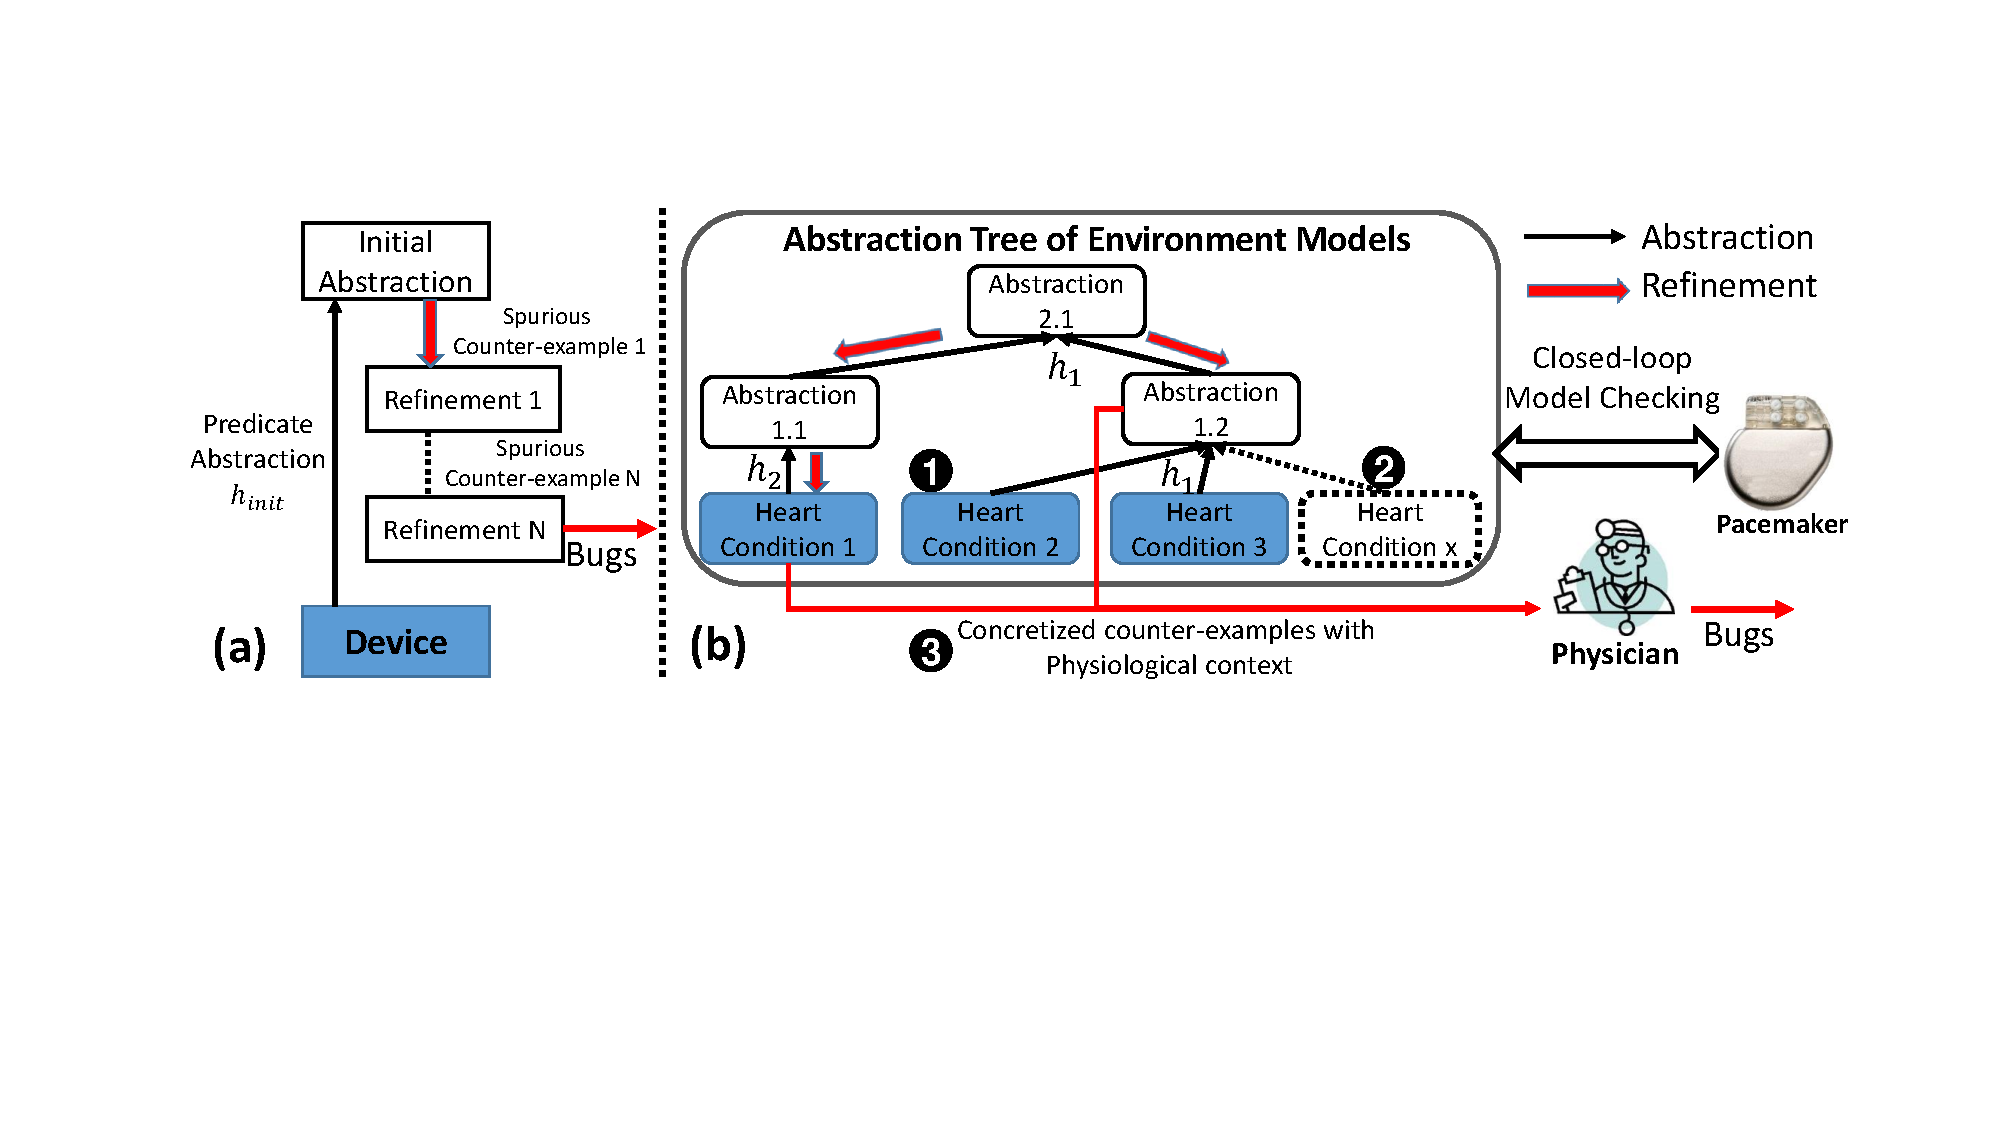
\includegraphics[width=\textwidth]{figs/distinction.pdf}
		%\vspace{-5pt}
		\caption{\small (a) Device modeling with CEGAR framework (b) Closed-loop model checking with environment abstraction tree.}% The initial set of heart conditions are first abstracted and/or merged using abstraction rules $h_1,h_2$ (Marker 1). The abstract model is first used for closed-loop model checking. When a property violation happens, refined models in the abstraction tree are used for model checking. The most concrete counter-examples may be available in the initial model(s) (Marker 2). In the scenario where counter-examples do not exist in explicitly modeled Heart condition 2 and 3, the counter-example in Abstraction 1.2 may correspond to a valid heart condition introduced during abstraction $h_1$. The physician decides the validity of the counter-examples.}
		  \vspace{-10pt}
		\label{fig:distinction}
\end{figure}


\subsection{Contributions}
In this paper a framework is proposed for environment modeling in closed-loop model checking of medical device software.
The cardiac pacemaker is used as an example of applying this framework.
An expandable set of timed-automata heart models are first developed to represent different physiological conditions (\figref{distinction} Marker 1).
A set of domain-specific abstraction rules are then developed based on physiological knowledge, which help ensure the physiological relevance of the behaviors introduced into the abstract models (\figref{distinction} Marker 2).
Then the rules are applied to the initial set of physiological models to obtain an abstraction tree, which will be used for closed-loop model checking of the pacemaker. 
A straightforward search procedure is then used to conduct model checking using suitable heart models and return the most concrete and unambiguous counter-examples to the physicians for analysis (\figref{distinction} Marker 3).
In this framework, physiological knowledge is only needed when constructing the initial model set and when analyzing counter-examples. 
The application of the physiological abstraction rules and the verification procedure can be automated.
The proposed method can potentially be generalized to other domains in which the device operates in a large variety of environmental conditions.
\subsection{Related Work}
%\todo[inline]{complete}
Counter-Example Guided Abstraction Refinement (CEGAR) \cite{CEGAR} has been proposed to over-approximate the behaviors of the device using predicate abstraction (\figref{distinction}.(a)).
%Upon property violation the abstract counter-example is checked for its validity on the actual system. If the counter-example is \emph{spurious} the model is then refined to eliminate the spurious counter-example. 
%This process is then continued on the refined model until either a valid counter-example returns or no counter-examples are returned. 
CEGAR works well during device modeling, however, it cannot be applied to environment modeling for two reasons: 1)~predicate abstraction does not guarantee the validity of behaviors introduced into the model. In fact, for device modeling, all additional behaviors introduced into the abstract model are spurious. 2)~the validity of a counter-example cannot be checked automatically as in device modeling. 

Proof-based approaches have also been applied to verify  abstractions and refinements of pacemaker specification using Event-B~\cite{eventb}. However, the authors did not take into account environment behaviors thus the framework cannot be used for verifying physiological requirements.  

Physiological modeling of cardiac activities has been studied at various levels for different applications. In \cite{natalia}, the electrical activity of the heart is modeled with high spatial fidelity to study the mechanisms of cardiac arrhythmia. In \cite{radu}, formal abstractions of cardiac tissue have been studied to reduce the complexity of the heart tissue model. However, these two models do not focus on the interaction with the pacemaker, therefore cannot be used for closed-loop model checking. In \cite{marta}, hybrid automata models of the heart has been used to capture the complex beat-to-beat dynamics of the heart tissue. However the model cannot be used to cover behaviors across different heart conditions.

In previous work \cite{sttt13} a set of formal heart models covering various heart conditions at different abstraction levels was developed, and closed-loop model checking was performed on models of implantable pacemakers. 
However, the physiological knowledge required during each step of closed-loop model checking prevents the method to be practical.


%During the closed-loop model checking, the most abstract model(s) that are appropriate to the requirement are automatically selected as the initial environment models. If the requirement is satisfied, the system is safe under the environment conditions covered by the initial environment models. If the requirement is violated in certain initial environment model, the children of the model in the abstraction tree are used for model checking until 1) the leaves of the tree is reached, or 2) there is no violations in the child nodes. The counter-examples obtained at the most refined models are returned to the physician for validity check. This process is automated so that no domain knowledge is required for the person who performs model checking. It also ensures the most concrete counter-examples with unambiguous physiological context are returned to the physician for analysis. 
%The first challenge in closed-loop model checking of pacemakers is that the human heart displays a large number of different conditions, henceforth referred to as `physiological conditions'.
%E.g., one heart may display \emph{atrial fibrillation} where the upper chambers of the heart (the atria) produce an exceedingly fast beat that prevents proper blood pumping.
%Another heart may display Premature Ventricular Contraction (PVC) where a location in the ventricles produces electrical impulses at erratic time instants.\Hao{I don't think these two conditions make sense to the reader}
%Each such condition will require its own formal model, and some models may display more than one condition.
%In this paper, we build such a set of formal heart models using the timed automata formalism in Section ???.
%Performing model checking with each model separately, we seek a method that can combine models, and perform model checking on the merged model. 
%The combination of models must be such that if the merged model is correct (according to the requirements) then so is every model that was combined into it.
%We present \emph{abstraction rules} in Section ?? which allow us to do precisely that.

%This initial set of models will necessarily be \emph{incomplete} because the number of physiological conditions is too large, and some of the conditions are too ill-understood for modeling.
%Thus, unlike system modeling in which one typically starts from one ground truth model to be verified, our starting point is an \emph{incomplete set of environment models}.
%Because of this incompleteness, we seek abstraction rules that introduce new \emph{physiologically meaningful} behavior which might actually be produced by heart models not in the initial set.
%These then correspond to heart conditions not taken explicitly into account. 
%This provides a second motivation for the domain-specific abstraction rules $R$ in Section ???, which can be thought of as relaxations of the conditions governing the model's behavior. 
%Like predicate abstraction, they produce models that over-approximate the behavior of the model they are applied to (i.e., $\beh(R(M)) \supset \beh(M)$).
%However, the new behavior they introduce might not be spurious. 
%We demonstrate such a case in Section ???.
%If model checking returns a counter-example on $R(M)$, the physician can decide whether this is actually physiologically plausible behavior and therefore the pacemaker needs to be debugged, or this is indeed spurious and should be thrown out (and the abstraction refined).
%
%Note this is different from classical predicate abstraction [???], which adds behavior in a domain-agnostic fashion. In fact, predicate abstraction is a fist step in the timed automata model checking procedure as presented in [ALur and Dill 1994].
%Our abstraction rules are used to combine and and abstract models \emph{prior} to model checking.
%%tttt
%
%\subsubsection{Contributions}
%In this paper we propose a framework for environment modeling and model checking of medical device software, in particular, pacemakers.
%Specifically, we present several extended timed automata models of various heart conditions in Section ???. 
%We define domain-specific abstraction rules for these models, and demonstrate how these can be applied to gradually add physiologically meaningful behavior in Section ???. 
%Using the models and the rules, we build an abstraction tree which serves to perform model checking of physiological requirements for the heart+pacemaker closed loop in Section ???.
%We illustrate the approach via case studies in Section ???, and conclude in Section ???
%

%

\section{Hybrid systems and simulations}
\label{sec:preliminaries}

This section presents fairly standard definitions on 
%transition systems, 
hybrid systems and their simulations \cite{AlurHLP00ieee}.
It also defines STORMED hybrid systems, which admit finite bisimulations \cite{VladimerouPVD08_STORMED}.

\subsection{Transition and hybrid systems}
\label{sec:transition systems}

%{\large Partitions.} Given a set $Q$, a \emph{partition} $\partition = \{P_1,\ldots,P_k\}$ of $Q$ is a set of disjoint subsets of $Q$ whose union equals $Q$. 
%Let $\equiv_\partition$ be the associated equivalence relation.
%Partition $\partition'$ \emph{refines} $\partition$ if every block $P'$ of $\partition'$ is a subset of some block $P$ of $\partition$; we write this as $\partition' \subset \partition$.
%
\begin{defn}
	\label{defn:transition system}
	A \emph{transition system} $T = (Q,\labelSet,\trans{},Q_0)$ consists of a set of states $Q$, a set of events $\labelSet$ , a transition relation $\trans{} \subset Q \times \labelSet \times Q$, a set of initial states $Q_0$. 
	We write $q \trans{\slabel}q'$ to denote a transition element $(q,\slabel,q') \in \trans{}$.
	Given $P\subset Q$, we define $Post_\slabel(P) \defeq \{q'\;|\;\exists q\in P. q \trans{\slabel}q'\}$
	%
	Given an equivalence relation $\sim$ on $Q$, the \emph{quotient system} $T/\sim$ is
	$T/\sim = (Q/\sim, \{*\}, \trans{}_\sim, Q_0/\sim)$
	where $[q] \trans{*}_\sim [q']$ iff $q \trans{\slabel} q'$ for some $\slabel \in \labelSet$.
	Here $[q]$ is the equivalence class of $q$ and $Q/\sim$ is the set of equivalence classes of $\sim$.
\end{defn}

\begin{defn}
	\label{defn:simulation}	
	Given two transition systems $T_1$ and $T_2$ with the same state space $Q$,
	a \emph{simulation} relation from $T_1$ to $T_2$ is a relation $\simu \subset Q \times Q$ such that 
	for all $(q_1,q_2) \in \simu$, if $q_1 \trans{\slabel}_1 q_1'$, there exists a $q_2' \in Q$ s.t. $q_2 \trans{\slabel}_2 q_2'$ and $(q_1',q_2') \in \simu$.
	A \emph{bisimulation relation} between $T_1$ and $T_2$ is both a simulation relation from $T_1$ to $T_2$ and from $T_2$ to $T_1$.
\end{defn}
%Given a partition $\partition$ of $Q$, the \emph{natural bisimulation} between $T$ and $T/\partition$ is $\Bc_P = \{(q,P) \in Q \times \partition \;|\; q \in P\}$.	
%Conversely, a bisimulation $\Bc$  of $T$ defines a partition $\partition_\Bc$ of $Q$ where $q,q'$ are in the same block of the partition iff $(q,q') \in \Bc$.
%
The bisimulation $\bisimu$ is said to \emph{respect} $\sim$ if $(q,q') \in \bisimu \implies q \sim q'$.
%
The following algorithm, if it terminates, yields a finite bisimulation for $T$ that respects the given equivalence relation~\cite{AlurHLP00ieee}.
Moreover, it is the \emph{coarsest} bisimulation (with respect to inclusion) that respects $\sim$.
\begin{algorithm}[t]
		\caption{Computing a bismimulation respecting $\sim$}
		\label{algo:bisimulation}
		\begin{algorithmic}
			\Require Transition system $T = (Q,\labelSet,\trans{},Q_0)$, equivalence relation $\sim$.
			\State Set $\simu = Q/\sim$			
			\While{$\exists P,P' \in \simu$ and $\slabel \in \labelSet$ s.t. $\emptyset \neq P' \cap Post_\slabel(P) \neq P'$}
				\State Set $\simu = \simu \setminus \{P'\} \cup \{P' \cap Post_\slabel(P) , P' \setminus Post_\slabel(P) \}$
			\EndWhile	
			\State Return $\simu$
		\end{algorithmic}
\end{algorithm}
Given a set of atomic propositions $AP$, if $\sim$ is s.t. $q \sim q'$ iff both states satisfy exactly the same set of atomic propositions, then model checking temporal logic properties can be done on the finite bisimulation instead of the possibly infinite $T$.
%The \emph{coarsest} bisimulation $\bisimu$ that refines a partition $\partition$ is one such that there is no other bisimulation $\bisimu'$ satisfying $\partition_\bisimu \subset \partition_{\bisimu'} \subset \partition$.

%Given a subset $P$ of $Q$, we define its $\slabel$-successor as $Post_\slabel(P) = \{q \in Q | \exists p \in P. q \trans{\slabel} p\}$.
%In other words, $Post_\slabel(P)$ is the set of states forward-reachable from $P$ via the event $\slabel$.


%
%Note that the resulting bisimulation is the \emph{coarsest} bisimulation (i.e., with the least number of blocks in its induced partition) that refines $\partition$.
%\subsection{Hybrid systems}
%\label{sec:hybridSystems}
\begin{defn}
	\label{defn:hybrid system}	
	A \emph{hybrid automaton} is a tuple \[\Sys = (\stSet,\modeSet,\hsSet_0,\{f_\mode\}, Inv,E, \{\reset_{ij}\}_{(i,j)\in E}, \{\guard_{ij}\}_{(i,j)\in E})\] where 
		 $\stSet \subset \Re^n$ is the continuous state space equipped with the Euclidian norm $\|\cdot\|$, 
		$\modeSet \subset \Ne$ is a finite set of modes,
		 $\hsSet_0 \subset \stSet \times \modeSet$ is an initial set,
		 $\{f_\mode\}_{\mode \in \modeSet}$ determine the continuous evolutions with unique solutions,
		 $Inv: \modeSet \rightarrow 2^\stSet$ defines the invariants for every mode,
		 $E \subset \modeSet^2$ is a set of discrete transitions,
		 \yhl{$\guard_{ij} \subset \stSet$ is guard set for the transitions (so $\Sys$ transitions $i \rightarrow j$ when $\stPt \in \guard_{ij}$),
		 $\reset_{ij}: \stSet \rightarrow \stSet$ is an edge-specific reset function.}
		 \\
		 Set $\hsSet = \modeSet\times \stSet$.
		 Given $(\mode,\stPt_0) \in \hsSet$, the \emph{flow} $\theta_{\mode}(;\stPt_0):\Re_+ \rightarrow \Re^n$ is the solution to the IVP $\dot{x}(t) = f_\mode (x(t))$, $\stPt(0)=\stPt_0$.
\end{defn}
%
The associated \emph{transition system} is $T_\Sys = (\hsSet,  E \cup \{\tau\},\trans{},\hsSet_0)$ 
where $\hsSet$ is the state set, $E \cup \{\tau\}$ is the label set for transitions, $\hsSet_0$ is the set of initial states, 
and $\trans{} = (\bigcup_{e \in E} \trans{e}) \cup \trans{\tau}$ 
where $(i,\stPt) \trans{e} (j,y)$ iff $e = (i,j), \stPt \in \guard_{ij}, y = \reset_{ij}(\stPt)$ and $(i,\stPt) \trans{\tau} (j,y)$ iff $i = j$ and there exists 
a flow $\theta_i(\cdot;x)$ of $\Sys$ and $t\geq 0$ s.t. $\theta_i(t;x)=y$ and $\forall t' \leq t$, $\theta_i(t';x) \in Inv(i)$.
%Note that the transition $\trans{\tau}$ abstracts away time, i.e. it doesn't preserve information about the duration of continuous flow.
%For a set $P \subset \hsSet$,$P_{|\stSet}$ denotes its projection onto $\stSet$, 
%and $P_{|\modeSet}$ its projection onto $\modeSet$. 
%\begin{defn}
%	\label{defn:reachability operators}[Reachability]
%	Let $\Sys$ be a hybrid system with hybrid state space $\hsSet$, 	 
%	$I = [0,b) \subset [0,+\infty)$ be a (possibly unbounded) interval, 
%	$t \in I$, 
%	and $\epsilon >0$.
%	The \emph{$\epsilon$-approximate continuous reachability operator}, 
%	$\Rc^{\epsilon}_t : 2^\hsSet \rightarrow 2^\hsSet$ is given by
%	\begin{eqnarray*}
%		\Rc^{\epsilon}_t(P) = \{(i,\stPt) \in \stSet | \exists x_0 \in P_{|\stSet}, t \geq 0. 
%		||\theta_i(t;x_0) - \stPt|| \leq \epsilon\} 
%	\end{eqnarray*}
%	where $P = \{i\}\times W$, $W \subset Inv(i)$.
%	%
%	Define also $\Rc^{\epsilon}_I(P) = \cup_{t\in I} \Rc^{\epsilon}_t(P)$.
%	%
%	The (exact) \emph{discrete reachability operator} is:
%	\begin{eqnarray*}
%	\Rc_{d}(P) &=& \cup_{j: (i,j) \in E} \reset_{ij}(P \cap G_{ij})
%	\end{eqnarray*}
%\end{defn}
%%
%For a hybrid system, $Post_\slabel$ computes the forward reach sets, and is implemented by $\Rc^0_{[0,\infty)}$ and $\Rc_d$. 
Let $\sim$ be an equivalence relation on $\hsSet$ and $\hsSet/\sim$ the corresponding partition.
Let $\Fc_t(\hsSet/\sim)$ be the coarsest bisimulation with respect to $\trans{\tau}$\footnote{I.e., $\Ft$ only considers the continuous transition relation: it is a bisimulation of $T_\Sys^c \defeq (\hsSet/\sim,\{*\},\trans{\tau},\hsSet_0/\sim)$.} 
respecting the partition $\hsSet/\sim$, 
and 
$\Fc_d(\hsSet/\sim) \defeq \{(h_1,h_2)  \;|\; (h_1 \trans{e} h_1') \implies (\exists e' \in E, h_2' \; . h_2 \trans{e'} h_2' \land h_1' \sim h_2') \} \cap \hsSet/\sim$ \cite{VladimerouPVD08_STORMED}.
The iteration 
\begin{eqnarray}
\label{eq:Ft,Fd}
W_0 = \Ft(\hsSet/\sim), \quad\forall i\geq 0,\; W_{i+1} = \Ft(\Fd(W_i))
\end{eqnarray}
computes a bisimulation of $\Sys$.
However it does not necessarily terminate for hybrid systems because the system's reach set might intersect a given block of $\hsSet/\sim$ an infinite number of times (see \cite{LaFerrierePS00_Ominimal} for an example).
The class of systems introduced in the next section has the property that the iteration does terminate for it and returns a finite $\simu$.

Given a set of atomic propositions, if $\sim$ is s.t. $\hsPt \sim \hsPt'$ iff both states satisfy exactly the same atomic propositions, then model checking temporal logic properties can be done on the finite bisimulation instead of the possibly infinite $\Sys$.

\subsection{O-minimality and STORMED systems}
\label{sec:ominimality}
We give a very brief introduction to o-minimal structures.
A more detailed introduction can be found in \cite{LaFerrierePS00_Ominimal}, and an exposition of topology and o-minimality in \cite{VanDerDriesBook}.
We are interested in sets and functions in $\Re^n$ that enjoy certain finiteness properties, called order-minimal sets (o-minimal).
These are defined inside \emph{structures} $\Ac = (\Re,<, +,-,\cdot,\exp,\ldots)$.
The subsets $Y \subset \Re^n$ we are interested in are those that are \emph{definable} using first-order formulas $\formula$: $Y = \{(a_1,\ldots,a_n) \in \Re^n \;|\;  \formula(a_1,\ldots,a_n)\}$.
(First-order formulas use the boolean connectives and the quantifiers $\exists,\forall$).
The atomic propositions from which the formulas are recursively built allow only the operations of the structure $\Ac$ on the real variables and constants, and the relations of $\Ac$ and equality.
For example $2x-3.6y < 3z$ and $x=y$ are valid atomic propositions of the structure $\Lc_\Re=(\Re,<, +,-,\cdot)$, while $cosh(x) < 3z$ is not because $cosh$ is not in the structure.
These structures are already sufficient to describe a set of dynamics rich enough for our purposes and for various classes of linear systems.
%\textbf{Formal definitions}.
A \emph{language} is a set of relations, functions and constants.
E.g. $\Lc_\Re = (<,+,-, \cdot,\Re)$ is the language where the only relation is $<$, the functions are $+,-,\cdot$, and the constants are taken from $\Re$,
and  $\Lc_{exp} = (<,+,-, \cdot,\exp, \Re)$ adds the exponential symbol to it.
Let $\Vc = \{x,y,z,x_1,x_2,\ldots\}$ be a set of variables.
A \emph{term} of a language is either a variable, a constant, or $F(\theta_1,\ldots,\theta_m)$ where $F$ is an $m$-ary function expressible in the language and the $\theta_i$ are terms.
E.g. $2x-3.6y$ is a term of $\Lc_\Re$.
The \emph{atomic formulas} of the language are of the form $\theta_1=\theta_2$ or $R(\theta_1,\ldots,\theta_m)$ where $R$ is an $m$-ary relation on the terms $\theta_i$.
E.g., $2x-3.6y < z\cdot z$ is a an atomic formula in $\Lc_\Re$ which uses the terms $2x-3.5y$ and $z \cdot z$.
The set of (first-order) \emph{formulas} is defined recursively as follows: every atomic formula is a formula, and if $\formula_1,\formula_2$ are formulas, then so are $\formula_1 \land \formula_2, \neg \formula_1, \forall x: \formula_1, \exists x:\formula_1$.
Here the symbols are the usual boolean connectives ( conjunction $\land$ and negation $\neg$), and quantifiers (there exists $\exists$ and for all $\forall$).
A \emph{sentence} in the language is a formula where all variables are inside the scope of a quantifier, e.g. $\exists y . (x+y>3)$ is not a sentence.

So far, a language has been defined in a purely syntactic manner.
A \emph{model} of a language is a set $S$ along with an interpretation of the relations, functions and constants of the language.
We are interested in this paper in the model of $\Lc_{exp}$ where the set $S = \Re$, and the symbols $<,+,-, \cdot,exp$ have their usual meaning (less than, addition, etc).
A set $Y \subset \Re^n$ is \emph{definable} in $\Lc_\Re$ if there exists a formula of the model such that $Y$ can be expressed as $Y = \{(a_1,\ldots,a_n) \in \Re^n \;|\; \formula(x_1,\ldots,a_n)\}$.
E.g., the formula $x^2-1=0$ defines the set $\{-1,+1\}$.
Finally, a \emph{theory} is a subset of sentences in the model $\Lc_\Re$, i.e. it is a collection of sentences that are true in $\Lc_\Re$.
\begin{defn}
	\label{defn:ominimal struct}	
	A theory of $(\Re,\ldots)$ is \emph{o-minimal} if the only definable subsets of $\Re$ are finite unions of points and (possibly unbounded) intervals.	
	A function $f:x \mapsto f(x)$ is o-minimal if its graph $\{(x,y) \;|\; y=f(x)\}$ is a definable set.
\end{defn}
We use the terms o-minimal and definable interchangeably, and they refer to the structure $\Lc_{\exp}= (\Re,<, +,-,\cdot,\exp)$, which is known to be o-minimal.
%
The dot product between $x,y\in \Re^n$ is denoted $x \cdot y$, and $d(Y,S)$ is the minimum distance between sets $Y$ and $S$.
\begin{defn}\cite{VladimerouPVD08_STORMED}.
	\label{defn:stormed system}	
	A \emph{STORMED hybrid system} (SHS) $\SHS$ is a tuple $(\Sys,\Ac, \phi,b_-,b_+, d_{min}, \epsilon,\zeta)$ where $\Sys$ is a hybrid automaton, $\Ac$ is an o-minimal structure, $d_{min}, \zeta \in \Re_+$, $b_-,b_+ \in \Re$ and $\phi \in \stSet^n$ such that:
	\\
	\textbf{(S)} The system is $d_{min}$-separable, meaning that for any $e=(\mode, \mode ')\in E$ and $\mode ''\neq \mode'$,$d(\reset_e(\guard_{(\mode ,\mode ')}), \guard_{(\mode' ,\mode '')})>d_{min}$
	\footnote{We updated the definition of separability from \cite{VladimerouPVD08_STORMED} to accurately capture the requirement that if $\Sys$ flows, it flows a uniform minimum distance along $\phi$. For this we need the starting point in the new mode, and any guard out of the mode, to be separated by at least $d_{min}$.}
%	for any two distinct edges $(\mode, \mode'), (\mode ,\mode '')$ in $E$, $\min\{||x_1 - x^2|| \;|\; x_1 \in G_{\mode, \mode'}, x_2 \in G_{\mode ,\mode ''}\} > d_{min}$
	\\
	\textbf{(T)} The flows (i.e., the solutions of the ODEs) are Time-Independent with the Semi-Group property (TISG), meaning that for any $\mode \in \modeSet, \stPt \in \stSet$, the flow $\theta_\mode$ starting at $(\mode , x)$ satisfies: 1) $\theta_{\mode}(0;x) = x$, 2) for every $t,t' \geq 0$, $\theta_{\mode}(t+t';x) = \theta_{\mode}(t'; \theta_\mode(t;x))$
	\\
	\textbf{(O)} All the sets and functions of $\Sys$ are definable in the o-minimal structure $\Ac$
	\\
	\textbf{(RM)} The resets and flows are monotonic with respect to the same vector $\phi$, meaning that \\
	1) (Flow monotonicity) for all $\mode \in \modeSet$, $x \in \stSet$ and $t,\tau \geq 0$, $\phi \cdot (\theta_\mode (t+\tau;x) - \theta_\mode (t;x) ) \geq \epsilon ||\theta_\mode (t+\tau;x) - \theta_\mode (t;x) ||$, 
	and \\
	2) (Reset monotonicity) for any edge $(\mode,\mode') \in E$ and any $x^-,x^+ \in \stSet$ s.t. $x^+ = R_{\mode ,\mode'}(x^-)$, 
	\begin{compactenum}
		\item if $\mode = \mode'$, then either $x^-=x^+$ or $\phi \cdot (x^+-x^-)\geq \zeta$
		\item if $\mode \neq \mode'$, then $\phi\cdot (x^+-x^-) \geq \epsilon ||x^+-x^-||$
	\end{compactenum}

	\textbf{(ED)} Ends are Delimited: for all $e \in E$ we have $\phi \cdot x \in (b_- , b_+)$ for all $x \in G_{e}$
\end{defn}
Intuitively, the above conditions imply the trajectories of the system always move a minimum distance along $\phi$ whether flowing or jumping, which guarantees that no area of the state space will be visited infinitely often. 
This is at the root of the finiteness properties of STORMED systems.
%
The following result justifies the interest in STORMED systems: they admit finite bisimulations.
\begin{thm}\cite{VladimerouPVD08_STORMED}
	\label{thm:stormed finite bisimu}	
	Let $\Sys$ be a STORMED hybrid system, and let $\partition$ be an o-minimal partition of its hybrid state space. 
	Then $\Sys$ admits a finite bisimulation that respects $\partition$.
\end{thm}
%We will need the following result.
%\begin{lemma}\cite{VladimerouPVD08_STORMED}
%	\label{lemma:finite steps}
%	Given a SHS $\SHS$, the number of discrete transitions of any execution of $\SHS$ is uniformly upper bounded.
%\end{lemma}
We need the following result in what follows.
\begin{prop}
	\label{prop:ED}
	If the state space $\stSet$ of a hybrid automaton $\Sys$ is bounded, then its guards have delimited ends.
\end{prop}
\begin{prf}
	For all guard sets $G$ and all $x \in G$, $||\phi \cdot x || \leq ||\phi|| \cdot ||x|| \leq ||\phi||.\max\{||x||, x\in \stSet \} < \infty$.
\end{prf}

	\vspace{-10pt}
\section{Formal Models of the Environment}
\label{formalModelsofEnv}
To perform closed-loop model checking of medical devices, formal models of their physiological environment are needed to represent different physiological conditions the devices may encounter. In this section, timed-automata \cite{timed_automata} models of the human heart are developed as the environment model for implantable pacemaker~\cite{sttt13,VHM_proc}. Physiological requirements are formalized with monitors and $ATCTL^*$ formula \cite{TCTL}. 
Model checking can then be performed on the closed-loop system in model checker UPPAAL \cite{uppaal}. %The physiological knowledge required during closed-loop model checking of medical devices are associated with the \emph{physiological models} and the \emph{physiological requirements}. It is thus important to maintain the physiological context of the models and link model behaviors to physiological requirements. In this section we use heart modeling as example to demonstrate physiological knowledge encoding. %First, we introduce the physiological basis for our heart modeling. Then we demonstrate our heart model structure which can be used to model different heart conditions. We link transitions in the models to physiological behaviors
 \begin{figure}[!t]
	\centering
	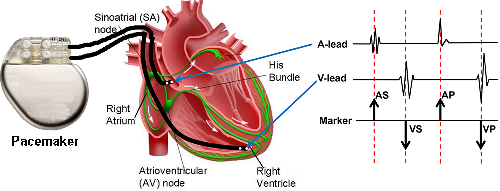
\includegraphics[width=0.7\textwidth]{figs/egm.pdf}
	
	%\vspace{-10pt}
	\caption{\small (a) Lead placement for a dual chamber pacemaker (b) Electrogram (EGM) signals from pacemaker leads and corresponding internal event markers}
	\label{fig:probes}
	\vspace{-10pt}
\end{figure} 

\subsection{Electrophysiological Heart Modeling Basics}
A healthy heart generates periodic electrical impulses to control heart rates according to physiological needs. 
These impulses propagate through the heart, triggering coordinated muscle contractions and pump blood to the rest of the body. 
The underlying pattern and timing of these impulses determine the heart's rhythm and are the key to proper heart functions. 
Derangements in this rhythm are referred to as \emph{arrhythmia}, which impair the heart's ability to pump blood and compromise the patients' health. 
Arrhythmias are categorized into so-called Tachycardia and Bradycardia. 
Tachycardia features undesirable fast heart rate which results in inefficient blood pumping. Bradycardia features slow heart rate which results in insufficient blood supply. Different heart conditions can be distinguished by the \emph{timing} of the electrical conduction, and the \emph{topology} of the electrical conduction system of the heart, which are researched in clinical setting referred to as \emph{Electrophysiology (EP)}\cite{josephson}. 
%Heart tissue can be modeled as \emph{Node automata} and the conduction delays between nodes are modeled as \emph{Path automata} (\figref{nodepathTA}). 
%\hatodoin{Last sentence repetitive?}


%\subsection{Timed-automata Models of the Heart}
%\label{labeledGraph}
%In a healthy heart, specialized tissue in the \emph{SA node} self-activate periodically. The signal conducts throughout both atria, causing them to contract and push the blood into the ventricles
%Models of different physiological conditions have to be developed to be able to interact with the medical devices. This initial set of physiological models should be able to distinguish the physiological conditions that each model represents. Ideally the models are developed using formalisms that are suitable for provable abstraction and model checking. 

%A node automaton models the conduction states of heart tissue, and changes therein. 
%Its three states correspond to 3 timing periods of the action potential. 
%From \textsf{Rest} state, the node can either self-activate or be activated by external stimuli (both events are indicated by Act\_node) and transition to the \textsf{ERP} state. 
%In the \textsf{ERP} state the node does not respond to external stimuli because it is refractory. 
%In the \textsf{RRP} state, the node can still be activated and transition to the \textsf{ERP} state.
%But the fact that the activation arrived early (in the RR Period) affects the ERP and the conduction delay of the tissue.  
%%This is tracked by a shared variable $C(i)$ for the $i^{th}$ node automaton. \todo[inline]{what is $C$?}
%%The new ERP period is determined by a function over clock value $g(f(t))$ which mimics the beat-to-beat dynamics described in \cite{josephson}. \todo[inline]{what are $g,f$?}
%
%The electrical conduction through the tissue \emph{between} nodes is abstracted using \emph{path automata}. 
%The path automata are used to represent structural or functional electrical connections between nodes. 
\begin{figure}[!t]
	\centering
	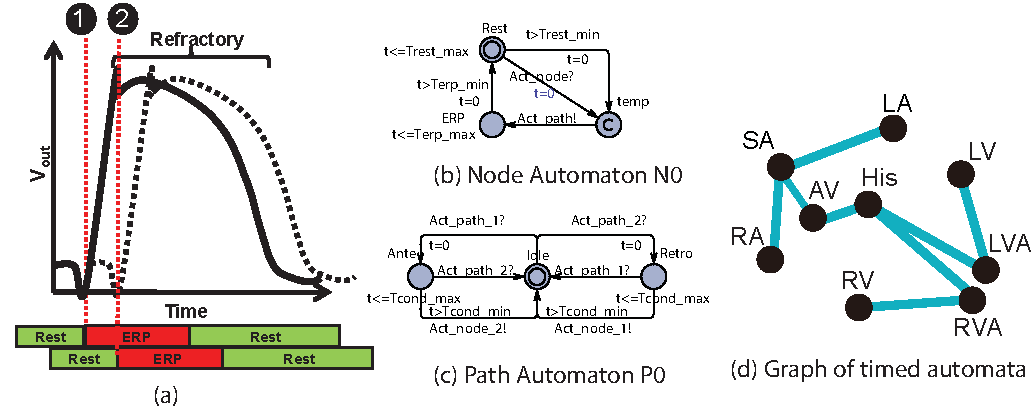
\includegraphics[width=0.9\textwidth]{figs/init_abs.pdf}
	\vspace{-10pt}
	\caption{\small (a) Action potential for a heart tissue and its tissue nearby (dashed). (b) Node automaton. (c) Path automaton. (d) An example model of the heart consist of a network of node and path automata. The nodes are labeled with the name of the corresponding physiological structures.}
	\vspace{-15pt}
	\label{fig:nodepathTA}
\end{figure}

%%At the same time the clock invariant of the state is modified according to the shared variable $C(a/b)$. 
%%This corresponds to the change of the conduction delay that is caused by early activation. 
%Similarly to a node automaton, the changing trend is extracted from clinical data. 
%
%The parameters of the node and path automata determine the ranges of time in which the automata can stay in corresponding locations. 
%The lower endpoint is specified as a clock invariant and the upper endpoint is specified as a guard. 
%For a heart model $G$ with $n$ nodes and $m$ paths (thus, $n$ vertices and $m$ edges), the node automata are denoted as $N_i, i\in[n]$ and path automata are denoted as $P_j,j\in[m]$. 
%\todo[inline]{change to $V_i$ and $E_i$ to stay consistent with definition of graph?}
%The parameters for the nodes are $Trest$ (with range $[Trest_{min}$),TERP,TRRP and the parameters for the paths are $\{Tante,Tretro\}$. 
<<<<<<< Updated upstream
=======
The spatial and temporal properties of a given human heart condition can be modeled by a network of node and path automata with different parameters (i.e., \figref{nodepathTA}.(d)). Physiological structures of the heart are represented as node automata and the path automata specify the connectivities of the nodes and the conduction delays among them. 
The network can be viewed as a labeled directed graph: %the vertices of the graph represent nodes, or locations, in the heart, while edges represent conduction paths between the nodes. 
\begin{defn}
	\label{def:labeledGraph}
	[Labeled graph]
	A \textbf{labeled graph} is a directed graph $G = (V,E,A)$ where 
	$V$ is a finite set of vertices, $E \subset V\times V$ is a finite set of directed edges,
	and $A$ is a total labeling function $A: V \cup E \rightarrow TA$
	where $TA$ is the set of timed automata.
	The function $A$ labels each vertex with a \emph{node automaton}, and each edge with an \emph{path automaton}.
	For a graph $G$, we write $\Ec(G) \defeq V(G) \cup E(G)$.
\end{defn}
The heart model structure has been used to model various heart conditions and all of them have been validated by electrophysiologists \cite{vhm_ecrts10}.
>>>>>>> Stashed changes

Implantable cardiac pacemakers are rhythm management devices designed to treat bradycardia. 
A typical dual chamber pacemaker has two leads inserted into the heart through the veins which can measure the local electrical activities of the right atrium and right ventricle, respectively. According to the timing between sensed impulses the pacemaker can deliver electrical pacing to the corresponding chamber to maintain proper heart rhythm (\figref{probes}).  

\subsection{Timed Automata Models of the Heart}
At cellular level, a heart tissue can be activated by an external voltage. Certain tissues also have the capability to self-activate, which contributes to natural heart beats. Once activated (Marker 1 in \figref{nodepathTA}), the voltage outside the tissue changes over time, which is referred to as \emph{Action Potential} (\figref{nodepathTA}.(a)). 
The action potential can be divided into two functional timing periods: The \emph{Effective Refractory Period (ERP)}, during which the tissue cannot be triggered by another activation; and the \emph{Rest} period, during which the tissue can be activated and at the end of which the tissue will self-activate. 
The timing behaviors of the action potential are modeled as \emph{node automaton} $A_v$ (\figref{nodepathTA}.(b)). 

A \textbf{node automaton} initializes with the \textsf{Rest} state.
From the \textsf{Rest} state, the node can either self-activate or be activated by external activations (indicated by Act\_node). 
Upon activation the node transition to the \textsf{ERP} state and activate all the paths connecting to the node (indicated by Act\_path). 
In the \textsf{ERP} state the node does not respond to external activations. 
At the end of \textsf{ERP} state the node transition to the \textsf{Rest} state. 
The duration a node automaton can stay in the \textsf{Rest} is in the range $[Trest\_min,Trest\_max]$, and the duration it can stay in \textsf{ERP} is in the range $[Terp\_min, Terp\_max]$.
For heart tissue without the capability to self-activate, the parameters $Trest\_min$ and $Trest\_max$ are set to $\infty$.
$Trest$ and $Terp$ are referred to as \emph{parameters} of the automaton $A_v$.

The voltage change of the heart tissue will activate the tissue nearby with certain delay (Marker 2 in \figref{nodepathTA}). 
This timing delay between heart tissue is modeled using \emph{path automata} $A_e$ (\figref{nodepathTA}.(c)). 
The initial state of a \textbf{path automaton} is \textsf{Idle}, which corresponds to no conduction. 
A path has two conduction directions, forward and backward.
These are represented by the states \textsf{Ante} and \textsf{Retro}, named after their standard physiological terms Antegrade and Retrograde.
If \textsf{Act\_path} event is received from one of the nodes (1 or 2) connected to the path, the transition to \textsf{Ante} or \textsf{Retro} state will occur in the path automaton. 
At the end of \textsf{Ante} and \textsf{Retro} state the path will transition to \textsf{Idle} state and send Act\_node signal to the node automaton connected to the other end of the path (2 or 1).
%The parameters of the path automaton $A_e$ are $Tcond$.
The spatial and temporal properties of a given human heart condition can be modeled by a network of node and path automata with different parameters (i.e., \figref{nodepathTA}.(d)). Physiological structures of the heart are represented as node automata and the path automata specify the connectivities of the nodes and the conduction delays among them. 
The network can be viewed as a labeled directed graph: %the vertices of the graph represent nodes, or locations, in the heart, while edges represent conduction paths between the nodes. 
\begin{defn}
	\label{def:labeledGraph}
	[Labeled graph]
	A \textbf{labeled graph} is a directed graph $G = (V,E,A)$ where 
	$V$ is a finite set of vertices, $E \subset V\times V$ is a finite set of directed edges,
	and $A$ is a total labeling function $A: V \cup E \rightarrow TA$
	where $TA$ is the set of timed automata.
	The function $A$ labels each vertex with a \emph{node automaton}, and each edge with an \emph{path automaton}.
	For a graph $G$, we write $\Ec(G) \defeq V(G) \cup E(G)$.
\end{defn}
The heart model structure has been used to model various heart conditions and all of them have been validated by electrophysiologists \cite{vhm_ecrts10,vhm_embc10}.
%The heart models used here are networks of node and path automata. The arrangement and density of nodes and paths differ for different conditions and levels of abstraction. 


%\subsection{Describe Model Behaviors with Physiological Context}
%During model abstractions, the abstract model covers all transitions of the more refined model. Transitions corresponding to physiological behaviors may be merged or replaced by other transitions. Without documenting these information, the abstract models lose their physiological context. 
%In the heart models we modeled physiological timing periods using locations in timed automata. The minimum time an automaton can stay in those locations is limited by the guard on a transition out of the location, and the maximum time is limited by the clock invariant of the state. 
%The transitions of heart tissue can be categorized into 3 basic transition groups:
%\begin{itemize}
%	\item \textbf{self:} The self-activation of the node automata. The \emph{min} and \emph{max} parameters equal to $Trest\_min$ and $Trest\_max$ parameters in the node automata, which specify the minimum and maximum intervals between consecutive self-activation events.
%
%	\item \textbf{block:} The blocking property of the node automata. The \emph{min} and \emph{max} parameters equal to $Terp\_min$ and $Terp\_max$ parameters in the node automata, which specify the minimum and maximum intervals between consecutive activations that can trigger path conduction.	
%	\item \textbf{cond:} The conduction property of the path automata. The \emph{min} and \emph{max} parameters equal to $Tcond\_min$ and $Tcond\_max$ parameters in the node automata, which specify the minimum and maximum delays between a node activation on one end and the activation on the other end.
%\end{itemize}
%As an example, a node automata $NA$ has two transition groups, which can be represented by $NA.self$ and $NA.block$
\begin{figure}[!t]
		\centering
		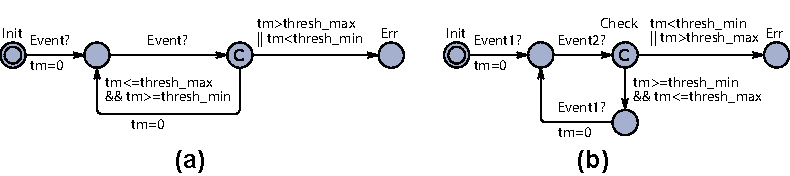
\includegraphics[width=0.8\textwidth]{figs/monitor.pdf}
		%\vspace{-5pt}
		\caption{\small (a) $M_{sing}$ for single event; (b) $M_{doub}$ for two events}
		  \vspace{-10pt}
		\label{fig:monitor}
\end{figure}
\subsection{Formalizing Physiological Requirements}
%Devices are designed to improve certain physiological conditions, the performance of the devices is evaluated on the difference between the patient conditions without the device and with the device. The device should also avoid deteriorating certain patient conditions, physiological requirements are specified in the form of:
%$$C_{pre}\rightarrow C_{post}$$
%in which $C_{pre}$ is the physiological conditions without the device,  and $C_{post}$ is the physiological condition with the device. For model-based closed-loop verification, $C_{pre}$ is often in form of a set of constraints on patient parameters. As a special case, $C_{pre}$ can equal to $true$, means that $C_{post}$ should be satisfied under all possible conditions.
%
%Physiological requirements are constraints on physiological behaviors. In \cite{iccps10} we 
%
%\subsection{Monitors}
Physiological requirements must be formalized for closed-loop model checking. In the case of medical devices, the devices are designed to \emph{improve} certain physiological conditions. 
%For an unhealthy open-loop physiological condition that a device is designed to improve, the closed-loop condition should be healthy.
Software developers are particularly interested in the scenario in which a healthy open-loop physiological condition became an unhealthy closed-loop condition due to device intervention, which is a bug in the device.

In general, a closed-loop requirement $\varphi$ is in the form of $\varphi_E\Rightarrow \varphi_C$, in which $\varphi_E$ is the open-loop physiological condition that the device encounters, often in form of parameter ranges in the environment models, and $\varphi_C$ is the closed-loop physiological condition that the device should achieve. Then we have:
\begin{equation}\label{req_def}
M_E\models\varphi_E \land M_E||M_D\models \varphi_C\Rightarrow M_E||M_D\models\varphi
\end{equation}
%\hatodoin{What is this comma in the equation? is is AND, or OR, or something else?}
%A requirement $\varphi: \varphi_E\Rightarrow \varphi_C$ contains open-loop environmental constraints in $\varphi_E$ and desired closed-loop condition specified in $\varphi_C$.  
The substates for a heart model are clocks and locations for each node and path automata. In \cite{vhm_iccps11}, physiological heart conditions are mapped to constraints on substate variables of the heart models, which can be written as atomic propositions. General monitors are also developed in Stateflow \cite{stateflow} for closed-loop testing of physiological requirements. The timed-automata version are shown in \figref{monitor}. The $M_{sing}(event,thresh\_min, thresh\_max)$ enforces the time interval between two $event$ signals within $[thresh\_min,thresh\_max]$. \\
$M_{doub}(event1,event2,thresh\_min,thresh\_max)$ enforces the time interval between $event1$ and $event2$ signals within $[thresh\_min,thresh\_max]$. Model checking is performed on the closed-loop system including the heart model $M_H$, the pacemaker model $M_P$, and the monitor $M$. The requirement $\varphi_P$ can be then represented with TCTL formula:
 \textsf{A[] (not M.Err)}

%%\subsection{State Space Formulation}
%\label{[statespaceformulation]}
%Kripke structure $<S,\Sigma,L,I>$ in which $S$ is a set of states, $\sigma(s_1,s_2)\in\Sigma\subset S^2$ is a set of transitions, $I\subset S$ is a non-empty set of initial states.
%
%To clarify things, we first introduce \emph{state groups} and \emph{transition groups}. The state space is defined by state variables. 
%$$s\{\theta_1,\theta_2\dots \theta_n\}\in S$$
%Each state $s$ is a valuation of all the state variables. Partial valuations can be used to represent a state group. For example, $s\{\theta_1=v_1\}$ represents all states in which $\theta_1=v_1$.
%
%Each state transition $\sigma\in\Sigma$ is defined as $\sigma(s_1,s_2)$ such that:
%$$s_1\xrightarrow{\sigma}s_2\text{ in which }s_1,s_2\in S$$
%Certain transitions have the same behaviors, mostly observablly equivalent . It is convinient to group them together to describe the behaviors of the system. A \textsf{transition group} is a group of transitions that the pre- and post- states satisfy certain criteria:
%$$\Sigma_\phi\subset\Sigma \text{ s.t. }\forall\sigma(s_1,s_2)\in\Sigma_\phi,f(s_1,s_2)\models\phi,s_1,s_2\in S$$
%in which $f(s_1,s_2)$ is certain proposition of the two states or their substates. It is possible that $\Sigma_{\phi_1}\cap\Sigma_{\phi_2}\neq \emptyset$.
%
%Ideal execution path of length n: $\delta:s_0\sigma_0\dots\sigma_i\dots\sigma_ns_n\in\Sigma^*$ in which: 
%$$s_0\in I, \sigma_i(s_i,s_{i+1})\in\Sigma, i\in[0,n-1]$$ 
%The set of all the transitions in a path is represented by $\Sigma_\delta$.
%
%Each transition takes time. We denote it as $t=T(\sigma)$. The time for each execution path: $$T(\delta)=\sum_{i=0}^nT(\sigma_i)$$
%
%Partial paths: Not all the transitions in a path are necessary. In fact, ideal paths are not possible, so do ideal models. One way to represent partial paths is timed execution path: sequence of transitions with unobservable ones abstracted with time lapse $\delta_t\in(\sigma_o,t)^*, t\in \mathbb{R}$
%
%$\delta_t$ is an abstraction of $\delta$, we denote it as $\delta\models\delta_t$. For a execution path 
%$$\delta=\sigma_0\sigma_1\dots\sigma_n$$
%there is a corresponding timed execution path 
%$$\delta^t=(\sigma_0^t,t_0)(\sigma_1^t,t_1)\dots(\sigma_m^t,t_m)$$ 
%in which
%$$\forall i,j,k \text{ s.t. } \sigma_i=\sigma_k^t,\sigma_j=\sigma_{k+1}^t,(\sigma_{i+1}\dots\sigma_{j-1})\neq\sigma_{j},T(\sigma_i\dots\sigma_j)=t_{k+1}-t_k$$
%with length $m<n$ such that $\delta\triangleleft\delta^t$. 
%
%Execution path produceable by model
%$$\delta\in^p M$$
%\subsection{A1: Observability Distinction}
%The lowest distinction requirement for a model
%
%The most basic observable transitions are input and output of the entity under modeling
%
%Input triggered transitions $\Sigma_i$
%
%Output inducing transitions $\Sigma_o$
%
%If we have a timed trace such that $\delta\triangleleft\delta_t$, all the transitions in a path $\delta$ which are input/output transitions should be preserved in the timed trace $\delta_t$. 
%%$$\delta\triangleleft\delta^t\rightarrow\forall \sigma\in(\Sigma_i\cup\Sigma_o)\cap\Sigma_\delta,\sigma\in\Sigma_(\delta_t)$$
%
%A model $M$ is observability distinctive iff
%$$\forall\delta^t\in^p M, \forall\delta\triangleleft\delta^t,\forall \sigma\in(\Sigma_i\cup\Sigma_o)\cap\Sigma_\delta,\sigma\in\Sigma_{\delta^t}$$
%The observability of the system and the environment are different. After the system has been developed, the observability of the environment is fixed. However, for the system itself, the observability can range from full white-box (code level) to full blackbox (input-output only)
%
%\subsection{A2: Property Distinction}
%We refer a model $M$ is property distinctive for property $\phi$ by $M\triangle\phi$, such that
%
%$$\forall \delta^t\in^p M, \delta^t\models\phi\leftrightarrow\forall \delta\triangleleft\delta^t,  \delta\models\phi$$
%%$$\forall \delta_1,\delta_2\triangleleft\delta_t, \delta_1\models\phi\leftrightarrow \delta_2\models\phi$$
%
%\subsection{A3: Validity Distinction}
%
%
%For system model $M^s$
%$$\delta^t\in^p M^s \text{ iff }\exists\delta\triangleleft\delta^t\text{ s.t. } \delta\in^p M^s$$
%
%
%There can be multiple execution path correspond to the same timed execution path. 
%$$\exists \delta_1,\delta_2\text{ s.t. } \delta_1\models\delta_t,\delta_2\models\delta_t$$
%In this case, we say that $\delta_1$ and $\delta_2$ are not \textbf{distinguishiable}. 
%
%Distinguishible transitions: a lot of the times two paths have to be distinguishible (healthy vs. unhealthy)
%
%
%Trace produceable by model: For an execution path $\delta$ with length $n$, we denote that the path is produceable by model $M$ with $\delta\triangleleft M$, such that:
%$$\forall \sigma(s_i,s_{i+1})\in \delta,i\in[0,n-1], s_0\in I, \sigma(s_i,s_{i+1})\in\Sigma_M$$
%
%Timed trace produceable by model:
%
%
%non-determinism
%
%For system:
%$$\delta\models\delta_t,\delta_t\triangleleft M_s \text {  iff  } \delta\triangleleft M_s$$
%For environment:
%$$\delta$$
%%\section{Model Abstraction With Over-approximation}
%%For two models $M_1$ and $M_2$, we denote $M_2$ is an abstraction of $M_1$ as $M_1\preceq M_2$. A function $s'=h(s),s\in S_1,s'\in S_2$ is a mapping from the states in $M_1$ to states in $M_2$. 
%%
%%For two models $M_1$ and $M_2$ such that $M_1\preceq M_2$, we know that all the transitions are preserved:
%%$$\forall \sigma(s,s') \in\Sigma_1\text{ s.t. }s,s'\in S_1,\rightarrow\sigma(h(s),h(s')) \in\Sigma_2,h(s),h(s')\in S_2$$
%%Due to the mapping the transition groups in $M_2$ are changed as well. For a transition group in $M_1$:
%%$$\Sigma_{\phi1}\subset\Sigma_1 \text{ s.t. }\forall\sigma(s_1,s_2)\in\Sigma_{\phi1},f(s_1,s_2)\models\phi1,s_1,s_2\in E_1$$
%In the more abstract model, the propsition is often relaxed. For certain $\phi2\supseteq\phi1$, we have:
%$$\Sigma_{\phi2}\subset\Sigma_2 \text{ s.t. }\forall\sigma(h(s_1),h(s_2))\in\Sigma_{\phi2},f(h(s_1),h(s_2))\models\phi2,s_1,s_2\in S_1$$
%
%
%Some of the transition groups are merged. For two transition groups $\Sigma_{\phi1},\Sigma_{\phi2}\subset\Sigma_1$ there exists a new relation $\Sigma_{\phi3}\subseteq\Sigma_2$ such that: $$\phi1\cup\phi2\subseteq\phi3$$
%We denote this abstraction as:
%$$\Sigma_{\phi3}=\{\Sigma_{\phi1},\Sigma_{\phi2}\}$$
%We use $\Sigma_{\phi1}\lhd\Sigma_{\phi3}$ to represent the abstraction relationship between transition groups.
%\begin{itemize}
	%\item Over-approximation and its information loss
    %\item Abstraction in terms of transition groups
    %
%\begin{itemize}
	%\item Merging
    %\item \textcolor{red}{Remove}
%\end{itemize}
	%\item Assumptions made to simplify the model and increase model behaviors
    %\item Necessity of model refinements due to information loss
%\end{itemize}
%
%\subsection{System model vs. Environment model}
%\begin{itemize}
	%\item System model achieves simplicity during abstraction
    %\item Environment model also use abstraction to achieve generalization
    %\item Validation of counter-example cannot be done on a generalized environment model
%\end{itemize}



\section{Physiological Abstraction rules}
\label{abstractionRules} 
In this section, domain-specific abstraction rules are developed that can introduce new behaviors to a given heart model or a set of models. 
These new behaviors are physiologically meaningful and might be manifested by a heart condition not explicitly modeled in the initial set of models.
The physician (or domain expert) remains the ultimate arbiter of what is physiologically meaningful.
This is a peculiarity of environment modeling, borne out of the fact that the initial set of models is necessarily incomplete, and does not represent all valid behaviors.
%We then show how the application of these domain-specific rules can be automated, thus obviating the need for domain expertise.

Recall that heart conditions are modeled as finite directed labeled graphs as introduced in Def.~\ref{def:labeledGraph}.
%Let $\Gc$ be the set of labeled graphs, and $2^\Gc$ be the power set of $\Gc$.
%An abstraction rule is a function $2^\Gc \rightarrow \Gc$.
Rules operate on a graph only if it has the appropriate structure for that rule, and if its parameters meet certain rule-specific conditions (if any).

\ifthenelse{\boolean{TECH_REPORT}}
{\subsubsection{Rule R1: Convert Reentry Circuits to Activation Nodes}
Within the conduction network of the heart, there can be multiple pathways between two locations, forming conduction loops. If the timing parameters of the tissue along the loop satisfy certain property, there can be scenarios in which an depolarization wave circling the circuit. The circuits are referred to as \emph{Reentry Circuits}. Since the time interval for an activation wave to circle a reentry circuit is usually less than the intrinsic heart cycle length, the heart rate will be "`hijacked"' by the reentry circuit once the cycling is triggered, causing tachycardia. Reentry is the most common mechanism for tachycardia which can be modeled by our heart models \cite{vhm_embc10}. 

The effect of reentry tachycardia is that activation signals coming out of the circuit with cycle length equals to the sum of conduction delays of the conduction paths forming the circuit. It is therefore reasonable to model a reentry circuit as a self-activation node with the self-activation range equal to the sum of conduction delays. \\
\textbf{Applicable Condition: } The rule only affect the topology of the model therefore can be applied without preliminaries.\\
\textbf{Output graph: }First detect the "essential structure" of the input graph, which are the shortest paths (in terms of conduction delay) connecting self-activation nodes and/or sensing nodes. Then detect all circles in the input graph. For each circle with nodes $N_i,i\in[1\dots n]$ and paths $P_j,j\in[1\dots m]$, remove all "non-essential" nodes and paths, create a node automaton $N_s$ and connect to the nearest sensing node with a path automaton $P_s$.\\
\textbf{Effect on parameters: }For the new node automaton $N_s$, we have :
$$N_s.TERP\_min=min(N_i.TERP\_min), N_s.TERP\_max=max(N_i.TERP\_max)$$
$$N_s.Trest\_min=\sum P_j.Tcond\_min,N_s.Trest\_max=\sum P_j.Tcond\_max$$
For the new path automaton $P_s$, assume the shortest path from $N_s$ to the nearest sensing node has paths $P_k,k\in[1\dots p]$, we have:
$$P_s.Tcond\_min=\sum P_k.Tcond\_min,P_s.Tcond\_max=\sum P_k.Tcond\_max$$
%For more complex structures with multiple circuits, the self-activation range will be the minimum of the shortest circuit to the maximum of the longest circuit. The detailed rule description and implementation can be found in %\cite{regar_tech}.
%\begin{figure}[!h]
%\centering
%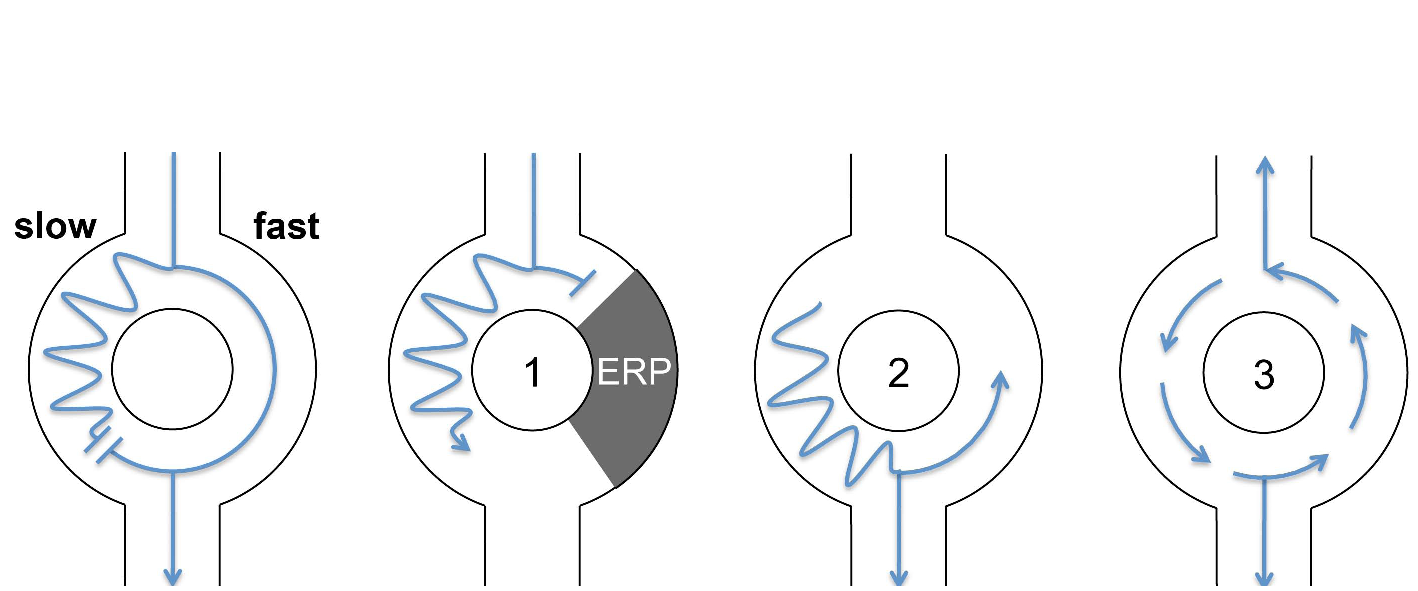
\includegraphics[width=0.6\textwidth]{figs/reentry.pdf}
%%\vspace{-5pt}
%\caption{\small Reentry Circuit}
%%\vspace{-15pt}
%\label{fig:reentry}
%\end{figure}
}
{Due to space limits only one abstraction rule is discussed in detail. The full set of rules and the proofs that these rules indeed produce over-approximations of the behavior space are relegated to the technical report \cite{regar_tech}.}
\ifthenelse{\boolean{TECH_REPORT}}
{\subsubsection{Rule R2: Remove Irrelevant Structures}
After the loops within the topology are removed, the topology of the heart model is in form of tree. Since the "non-essential" structure do not affect the activation signals from and/or to the sensing nodes, all the "non-essential" structure can be then removed.\\
\textbf{Applicable Conditions: }The rule can be applied after Rule 1 has been applied.\\
\textbf{Output Graph: } Trimmed graph with only essential structure remaining.\\
\textbf{Effects on parameters: } There is no effects on parameters of the node and path automata.
 
%\todo[inline]{Not true. Teh behavior is affected. Because this is a formal methods conference, so behavior and so on mean very specific things.}
\subsubsection{Rule R3: Removing Unnecessary Non-self-activation Nodes}
The effect of non-self-activation nodes is blocking electrical events with interval shorter than its ERP period. If the self-activation nodes at both ends of a core path have self-activation interval longer than the maximum ERP period of nodes along the core path, the nodes can be removed.\\
\textbf{Applicable Conditions: } This rule can be applied when there is no circles  in the heart model (Rule 1 has been applied).\\
\textbf{Output Graph: } For any structure $P_1-N_n-P_2$ which $N_n$ is a non-self-activation node, if $N_n.ERP_{max}<min(N_1.Rest_{min},N_2.Rest_{min})$, replace $P_1-N_n-P_2$ with $P_3$\\
\textbf{Effects on parameters: }
$$P_3.cond_{min}=P_1.cond_{min}+P_2.cond_{min}$$
$$P_3.cond_{max}=P_1.cond_{max}+P_2.cond_{max}$$

\subsubsection{Rule R4: Merge Parameter Ranges}
Timing periods of heart tissue, like Rest and ERP, are modeled as locations in the node and path automata. 
The minimum and maximum time an automaton can stay in a location is governed by the parameters in the guards and invariants. 
By expanding these periods, we introduce new behavior where a heart may stay in Rest for longer, or (self-)activate a node faster, etc.
\\
\textbf{(Sub)graph(s) to which it applies}.
This rule applies to a set of graphs $G_i$ with the same structure (i.e., they are pairwise isomorphic) but possibly with different parameters: $R(G_1,\ldots,G_n) = G'$.
See Fig.~\ref{fig:HM_abs}.\\
\textbf{Applicability conditions}.
None.\\
\textbf{Output (sub)graph}.
$G'$ has the same structure as the $G_i$.
Thus there's an isomorphism $f$ between every $G_i$ and $G'$.
Given an element $x$ of $G'$, $f^{-1}(x') = \{x_1,\dots,x_n\}$ are used to represent the set of elements that map to it via $f$, where $x_i \in \Ec(G_i)$.\\
\textbf{Effect on parameters}
%Recall Def.~\ref{def:labeledGraph}
For every automaton $A(x'), x' \in \Ec(G')$, and every parameter $\theta^{x'}$ of $A(x')$, 
$\theta_{min}^{x'} = \min(\theta^x_{min})_{x \in f^{-1}(x') }$ and 
$\theta_{max}^{x'} = \max(\theta^x_{max})_{x \in f^{-1}(x') }$}
{}
%\subsubsection{Rule R1: Convert Reentry Circuits to Activation Nodes}
Within the conduction network of the heart, there can be multiple pathways between two locations, forming conduction loops. If the timing parameters of the tissue along the loop satisfy certain property, there can be scenarios in which an depolarization wave circling the circuit. The circuits are referred to as \emph{Reentry Circuits}. Since the time interval for an activation wave to circle a reentry circuit is usually less than the intrinsic heart cycle length, the heart rate will be "`hijacked"' by the reentry circuit once the cycling is triggered, causing tachycardia. Reentry is the most common mechanism for tachycardia which can be modeled by our heart models \cite{vhm_embc10}. 

The effect of reentry tachycardia is that activation signals coming out of the circuit with cycle length equals to the sum of conduction delays of the conduction paths forming the circuit. It is therefore reasonable to model a reentry circuit as a self-activation node with the self-activation range equal to the sum of conduction delays. \\
\textbf{Applicable Condition: } The rule only affect the topology of the model therefore can be applied without preliminaries.\\
\textbf{Output graph: }First detect the "essential structure" of the input graph, which are the shortest paths (in terms of conduction delay) connecting self-activation nodes and/or sensing nodes. Then detect all circles in the input graph. For each circle with nodes $N_i,i\in[1\dots n]$ and paths $P_j,j\in[1\dots m]$, remove all "non-essential" nodes and paths, create a node automaton $N_s$ and connect to the nearest sensing node with a path automaton $P_s$.\\
\textbf{Effect on parameters: }For the new node automaton $N_s$, we have :
$$N_s.TERP\_min=min(N_i.TERP\_min), N_s.TERP\_max=max(N_i.TERP\_max)$$
$$N_s.Trest\_min=\sum P_j.Tcond\_min,N_s.Trest\_max=\sum P_j.Tcond\_max$$
For the new path automaton $P_s$, assume the shortest path from $N_s$ to the nearest sensing node has paths $P_k,k\in[1\dots p]$, we have:
$$P_s.Tcond\_min=\sum P_k.Tcond\_min,P_s.Tcond\_max=\sum P_k.Tcond\_max$$
%For more complex structures with multiple circuits, the self-activation range will be the minimum of the shortest circuit to the maximum of the longest circuit. The detailed rule description and implementation can be found in %\cite{regar_tech}.
%\begin{figure}[!h]
%\centering
%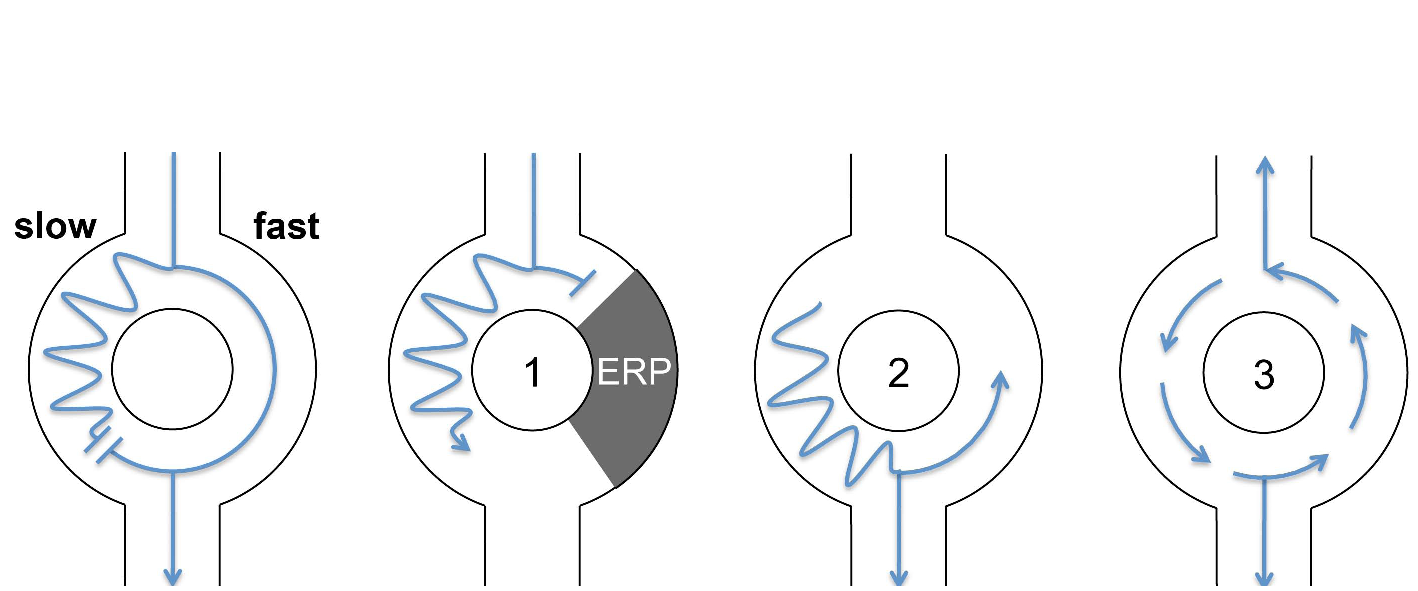
\includegraphics[width=0.6\textwidth]{figs/reentry.pdf}
%%\vspace{-5pt}
%\caption{\small Reentry Circuit}
%%\vspace{-15pt}
%\label{fig:reentry}
%\end{figure}

%\subsubsection{Rule R2: Remove Irrelevant Structures}
After the loops within the topology are removed, the topology of the heart model is in form of tree. Since the "non-essential" structure do not affect the activation signals from and/or to the sensing nodes, all the "non-essential" structure can be then removed.\\
\textbf{Applicable Conditions: }The rule can be applied after Rule 1 has been applied.\\
\textbf{Output Graph: } Trimmed graph with only essential structure remaining.\\
\textbf{Effects on parameters: } There is no effects on parameters of the node and path automata.
 
%\todo[inline]{Not true. Teh behavior is affected. Because this is a formal methods conference, so behavior and so on mean very specific things.}
\subsubsection{Rule R3: Removing Unnecessary Non-self-activation Nodes}
The effect of non-self-activation nodes is blocking electrical events with interval shorter than its ERP period. If the self-activation nodes at both ends of a core path have self-activation interval longer than the maximum ERP period of nodes along the core path, the nodes can be removed.\\
\textbf{Applicable Conditions: } This rule can be applied when there is no circles  in the heart model (Rule 1 has been applied).\\
\textbf{Output Graph: } For any structure $P_1-N_n-P_2$ which $N_n$ is a non-self-activation node, if $N_n.ERP_{max}<min(N_1.Rest_{min},N_2.Rest_{min})$, replace $P_1-N_n-P_2$ with $P_3$\\
\textbf{Effects on parameters: }
$$P_3.cond_{min}=P_1.cond_{min}+P_2.cond_{min}$$
$$P_3.cond_{max}=P_1.cond_{max}+P_2.cond_{max}$$

\subsubsection{Rule R4: Merge Parameter Ranges}
Timing periods of heart tissue, like Rest and ERP, are modeled as locations in the node and path automata. 
The minimum and maximum time an automaton can stay in a location is governed by the parameters in the guards and invariants. 
By expanding these periods, we introduce new behavior where a heart may stay in Rest for longer, or (self-)activate a node faster, etc.
\\
\textbf{(Sub)graph(s) to which it applies}.
This rule applies to a set of graphs $G_i$ with the same structure (i.e., they are pairwise isomorphic) but possibly with different parameters: $R(G_1,\ldots,G_n) = G'$.
See Fig.~\ref{fig:HM_abs}.\\
\textbf{Applicability conditions}.
None.\\
\textbf{Output (sub)graph}.
$G'$ has the same structure as the $G_i$.
Thus there's an isomorphism $f$ between every $G_i$ and $G'$.
Given an element $x$ of $G'$, $f^{-1}(x') = \{x_1,\dots,x_n\}$ are used to represent the set of elements that map to it via $f$, where $x_i \in \Ec(G_i)$.\\
\textbf{Effect on parameters}
%Recall Def.~\ref{def:labeledGraph}
For every automaton $A(x'), x' \in \Ec(G')$, and every parameter $\theta^{x'}$ of $A(x')$, 
$\theta_{min}^{x'} = \min(\theta^x_{min})_{x \in f^{-1}(x') }$ and 
$\theta_{max}^{x'} = \max(\theta^x_{max})_{x \in f^{-1}(x') }$
\ifthenelse{\boolean{TECH_REPORT}}
{\subsubsection{Rule R5: Merge Self-activation Nodes with Interaction Nodes}
%\todo[inline]{not clear}
The effect of self-activation nodes on the interaction of the pacemaker is triggering sensing events within certain delay. In this rule we merge all the self-activation nodes to their nearest interaction nodes. \\
\textbf{Applicability conditions: }The rule can be applied after all the non-activating nodes are removed.\\
\textbf{Output graph: }Assume the set of sensing nodes are $N_s^i$ and the set of self-activating nodes are $N_a^j$. The minimum timing delay between two nodes are the sum of conduction delay of the path automata along the path, which we denote as $dist(N_1,N_2)$. Each self-activating nodes $N_a$ is merged with the nearest sensing node $i=arcmin_i(dist(N_s^i,N_a))$.\\
\textbf{Effects on parameters: }Assume $N_a^i$ is the set of self-activating nodes that are merged with sensing node $N_s^i$. The parameters of $N_s^i$ are decided by:
$$N_s^i.TERP\_min=min(N_a^i.TERP\_min), N_s^i.TERP\_max=max(N_a^i.TERP\_max)$$
$$N_s^i.Trest\_min=min(N_a^i.Trest\_min), N_s^i.Trest\_max=max(N_a^i.Trest\_max)$$

\subsubsection{Rule R6: Replace Blocking With Non-deterministic Conduction}
%\todo[inline]{in modeling section mention self-activating and passive nodes}
%If a node automaton is in its \textsf{ERP} state, a \textsf{Act\_node} event is "blocked" and will not trigger corresponding path conduction. If we add non-deterministic transitions to the path automata such that a \textsf{Act\_path} event do not trigger state transitions to \textsf{ante} or \textsf{retro} (\figref{rule5}), the blocking behavior of the node is covered. We can then merge the \textsf{ERP} state with the \text{Rest} state in the node automata, and all passive nodes can be removed. An application of Rule 6 is shown in \figref{abs_exam}.\\
Consider the structure $N_1 P_1 N_2 P_2 N_3$ with three nodes and two paths, where $N_2$ is a passive node (i.e. not self-activating).
If $N_2$ blocks an activation signal from $N_1$ to $N_3$, this is equivalent to the paths $P_1$ or $P_2$ not conducting.
In this rule, the structure $P_1 N_2 P_2$ is replaced by a path $P$ whose automaton can take a self loop when it receives an activation signal, thus effectively stopping the conduction. 
This is shown in Fig.~\ref{fig:rule5}: the extra transitions are marked Act\_path\_1? and Act\_path\_2?.
Because the blocking effect of nodes is now incorporated into the paths, the node automata of self-activating nodes can be modified to the one shown in Fig.~\ref{fig:rule5}, which doesn't have the (now useless) ERP period.
\\
\textbf{Subgraph to which it applies}.
Line graphs with 3 vertices $N_1 P_1 N_2 P_2 N_3$, and self-activating nodes.\\
\textbf{Applicability conditions}
$N_2$ is a passive node.\\
\textbf{Output subgraph}.
$N'_1 P' N'_3$
A path $P'$ whose path automaton is as shown in Fig.~\ref{fig:rule5}.b.
The self-activating nodes $N$ are replaced by nodes $N'$ with automata shown in Fig.~\ref{fig:rule5}.a.\\
\textbf{Effect on parameters}
For the new path, $P.cond_{min}=P_1.cond_{min}+P_2.cond_{min}$ and 
$P.cond_{max}=P_1.cond_{max}+P_2.cond_{max}$
For the new nodes, $N'.Trest_{min}=N.Terp_{min}+N.Trest_{min}$ and 
$N'.Trest_{max}=N.Terp_{max}+N.Trest_{max}$.\\
\subsubsection{Interaction With the Pacemaker}
The interactions between the heart and the pacemaker are modeled by using binary event channels. For the atrial lead, we have:
\textsf{$N_A.Act\_path!\rightarrow$AS!},
and for ventricular lead we have
\textsf{$N_V.Act\_path!\rightarrow$VS!}.\\
The pacemaker accordingly generates atrial or ventricular pacing actions \textsf{AP!$\rightarrow N_A.Act\_node!$} and \textsf{VP!$\rightarrow N_V.Act\_node!$}.}
{}


%\subsubsection{Rule R5: Merge Self-activation Nodes with Interaction Nodes}
%\todo[inline]{not clear}
The effect of self-activation nodes on the interaction of the pacemaker is triggering sensing events within certain delay. In this rule we merge all the self-activation nodes to their nearest interaction nodes. \\
\textbf{Applicability conditions: }The rule can be applied after all the non-activating nodes are removed.\\
\textbf{Output graph: }Assume the set of sensing nodes are $N_s^i$ and the set of self-activating nodes are $N_a^j$. The minimum timing delay between two nodes are the sum of conduction delay of the path automata along the path, which we denote as $dist(N_1,N_2)$. Each self-activating nodes $N_a$ is merged with the nearest sensing node $i=arcmin_i(dist(N_s^i,N_a))$.\\
\textbf{Effects on parameters: }Assume $N_a^i$ is the set of self-activating nodes that are merged with sensing node $N_s^i$. The parameters of $N_s^i$ are decided by:
$$N_s^i.TERP\_min=min(N_a^i.TERP\_min), N_s^i.TERP\_max=max(N_a^i.TERP\_max)$$
$$N_s^i.Trest\_min=min(N_a^i.Trest\_min), N_s^i.Trest\_max=max(N_a^i.Trest\_max)$$

\subsubsection{Rule R6: Replace Blocking With Non-deterministic Conduction}
%\todo[inline]{in modeling section mention self-activating and passive nodes}
%If a node automaton is in its \textsf{ERP} state, a \textsf{Act\_node} event is "blocked" and will not trigger corresponding path conduction. If we add non-deterministic transitions to the path automata such that a \textsf{Act\_path} event do not trigger state transitions to \textsf{ante} or \textsf{retro} (\figref{rule5}), the blocking behavior of the node is covered. We can then merge the \textsf{ERP} state with the \text{Rest} state in the node automata, and all passive nodes can be removed. An application of Rule 6 is shown in \figref{abs_exam}.\\
Consider the structure $N_1 P_1 N_2 P_2 N_3$ with three nodes and two paths, where $N_2$ is a passive node (i.e. not self-activating).
If $N_2$ blocks an activation signal from $N_1$ to $N_3$, this is equivalent to the paths $P_1$ or $P_2$ not conducting.
In this rule, the structure $P_1 N_2 P_2$ is replaced by a path $P$ whose automaton can take a self loop when it receives an activation signal, thus effectively stopping the conduction. 
This is shown in Fig.~\ref{fig:rule5}: the extra transitions are marked Act\_path\_1? and Act\_path\_2?.
Because the blocking effect of nodes is now incorporated into the paths, the node automata of self-activating nodes can be modified to the one shown in Fig.~\ref{fig:rule5}, which doesn't have the (now useless) ERP period.
\\
\textbf{Subgraph to which it applies}.
Line graphs with 3 vertices $N_1 P_1 N_2 P_2 N_3$, and self-activating nodes.\\
\textbf{Applicability conditions}
$N_2$ is a passive node.\\
\textbf{Output subgraph}.
$N'_1 P' N'_3$
A path $P'$ whose path automaton is as shown in Fig.~\ref{fig:rule5}.b.
The self-activating nodes $N$ are replaced by nodes $N'$ with automata shown in Fig.~\ref{fig:rule5}.a.\\
\textbf{Effect on parameters}
For the new path, $P.cond_{min}=P_1.cond_{min}+P_2.cond_{min}$ and 
$P.cond_{max}=P_1.cond_{max}+P_2.cond_{max}$
For the new nodes, $N'.Trest_{min}=N.Terp_{min}+N.Trest_{min}$ and 
$N'.Trest_{max}=N.Terp_{max}+N.Trest_{max}$.\\
\subsubsection{Interaction With the Pacemaker}
The interactions between the heart and the pacemaker are modeled by using binary event channels. For the atrial lead, we have:
\textsf{$N_A.Act\_path!\rightarrow$AS!},
and for ventricular lead we have
\textsf{$N_V.Act\_path!\rightarrow$VS!}.\\
The pacemaker accordingly generates atrial or ventricular pacing actions \textsf{AP!$\rightarrow N_A.Act\_node!$} and \textsf{VP!$\rightarrow N_V.Act\_node!$}.



\begin{figure}[!b]
	\centering
	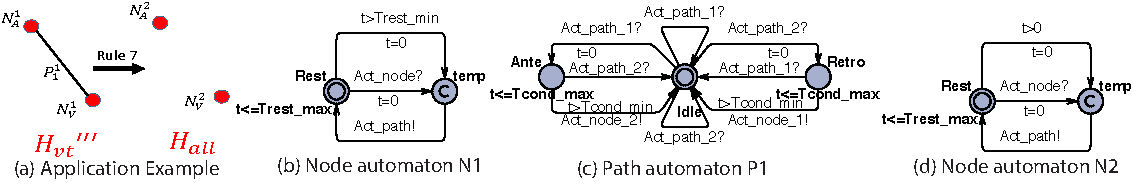
\includegraphics[width=1.05\textwidth]{figs/rule5.pdf}
	%\vspace{-5pt}
	\caption{\small (a) Rule 7 application example; (b)(c) Node and path automata used in $H_{vt}'''$; (d) Node automata used in $H_{all}$ }
	\vspace{-15pt}
	\label{fig:rule5}
\end{figure}

\subsubsection{Rule R7: Replace Conduction With Self-activation}
We describe Rule R7 as it illustrates both effects of an abstraction rule: structure change and modifications to the automata.
The effect of a conduction path is to conduct electrical activity from a node. Since the pacemaker cannot distinguish self-activation of the node and activation triggered by path conduction, we can use self-activation to replace path conduction.
If all self-activation nodes are allowed at any time by setting their minimum Rest period to 0, all the conduction paths can be removed, while preserving the original behaviors (where the Rest period was constrained to a finite interval).\\
\textbf{Applicability conditions}.
This rule can only be applied after Rule 5 and Rule 6 have been applied.\\
\textbf{Output graph}.
All edges are deleted: $G' = (V(G), \emptyset)$. The node automata are replaced with the one shown in \figref{rule5}.d.\\
\textbf{Effect on parameters}
For every node automaton $N$ in $G'$, $N.Trest_{min}=0$.\\

Consider \figref{rule5}.(a) showing an application of R7, $H_{vt}'''=N^1_AP^1N^1_V$ is abstracted to $H_{all}=N^2_AN^2_V$. Here we prove that $H_{vt}'''\preceq_t H_{all}$ with observable events $\Sigma_o=\{N_A.Act\_path,N_V.act\_path\}$. The state of $H_{vt}'''$ is represented by $(N^1_A.loc,P^1_1.loc,N^1_V.loc,N^1_A.t,P^1_1.t,N^1_V.t)$ and the state of $H_{all}$ is represented by $(N^2_A.loc,N^2_V.loc,N^2_A.t,N^2_V.t)$. Due to space limit, only one transition from each category is presented:\\
\textbf{Initial state: }First for the initial state we have:
$$\left\langle (Rest,Idle,Rest,0,0,0),(Rest,Rest,0,0)\right\rangle\in sim_o$$ 
\textbf{Timed transitions: }Consider a timed transition in $H_{vt}'''$
$$(Rest,Idle,Rest,t_1,t_2,t_3)\xrightarrow[]{\tau}(Rest,Idle,Rest,t_1+\tau,t_2+\tau,t_3+\tau)$$
in which $(\tau\in\mathbb{R})\wedge (t_1+\tau\leq N^1_A.Trest\_max)\wedge( t_3+\tau\leq N^1_V.Trest\_max)$. For a state in $H_{all}$ such that $\left\langle (Rest,Idle,Rest,t_1,t_2,t_3),(Rest,Rest,t_1,t_3)\right\rangle\in sim_o$,  there is a timed transition:
$$(Rest,Rest,t_1,t_3)\xrightarrow[]{\tau}(Rest,Rest,t_1+\tau,t_3+\tau)$$
and $\left\langle (Rest,Idle,Rest,t_1+\tau,t_2+\tau,t_3+\tau),(Rest,Rest,t_1+\tau,t_3+\tau)\right\rangle\in sim_o$.\\
%The state of $H_{vt}'''$ is given by the locations of the three automata.
%$$(Rest,Idle,Rest,[Trest\_min, Trest\_max]$$
%$$(Rest,Idle,Rest)\xrightarrow[]{N^1_A.t<N^1_A.Trest\_min \wedge N^1_V.t<N^1_V.Trest\_min}(Rest,Idle,Rest)$$
%are mapped to the following transition in $H_{all}$:
%$$(Rest,Rest)\xrightarrow[]{N^2_A.t<N^2_A.Trest\_min \wedge N^2_V.t<N^2_V.Trest\_min}(Rest,Rest)$$
%
%Self-activations of the atrial node:
%$$(Rest,Idle,Rest,t_1,t_2,t_3)\xrightarrow[\textcolor{red}{N^1_A.Act\_path!}]{t_1\in [N^1_A.Trest\_min, N^1_A.Trest\_max] }(Rest,Ante,0,0,t_3)$$
%are mapped to the following transition in $H_{all}$:
%$$(Rest,Rest,t_1,t_3)\xrightarrow[\textcolor{red}{N^2_A.Act\_path!}]{t_1\in [0, N^2_A.Trest\_max]}(Rest,Rest,0,t_3)$$
%Self-activations of the ventricular node:
%$$(Rest,Idle,Rest,t_1,t_2,t_3)\xrightarrow[\textcolor{red}{N^1_V.Act\_path!}]{t_3\in [N^1_V.Trest\_min, N^1_V.Trest\_max] }(Rest,Retro,Rest,t_1,0,0)$$
%are mapped to the following transition in $H_{all}$:
%$$(Rest,Rest,t_1,t_3)\xrightarrow[\textcolor{red}{N^2_V.Act\_path!}]{t_3\in [0, N^2_V.Trest\_max]}(Rest,Rest,t_1,0)$$
\textbf{Discrete transitions: }Consider a discrete transition in $H_{vt}'''$
$$(Rest,Ante,Rest,t_1,t_2,t_3)\xrightarrow[t_2\in [P^1_1.Tcond\_min, P^1_1.Tcond\_max) ]{\textcolor{red}{N^1_V.Act\_path!}}(Rest,Idle,Rest,t_1,t_2,0)$$
in which $N^1_V.Act\_path!\in\Sigma_o$. \\
For a state in $H_{all}$ such that $\left\langle (Rest,Idle,Rest,t_1,t_2,t_3) ,(Rest,Rest,t_1,t_3)\right\rangle\in sim_o$,  there is a discrete transition:
$$(Rest,Rest,t_1,t_3)\xrightarrow[t_3\in [0, N^2_V.Trest\_max)]{\textcolor{red}{N^2_V.Act\_path!}}(Rest,Rest,t_1,0)$$
and $\left\langle ((Rest,Idle,Rest,t_1,t_2,0)),(Rest,Rest,t_1,0)\right\rangle\in sim_o$. Basically activation due to conduction is replaced by self-activation of the corresponding node automata.\\
\textbf{Additional behaviors: }The timed-simulation also allows additional behaviors into $H_{all}$. Consider a discrete transition in $H_{all}$
$$(Rest,Rest,t_1,t_3)\xrightarrow[t_3\in [0, N^2_V.Trest\_min)]{\textcolor{red}{N^2_V.Act\_path!}}(Rest,Rest,t_1,0)$$
However, for a state in $H_{vt}'''$ such that $\left\langle (Rest,Idle,Rest,t_1,t_2,t_3),(Rest,Rest,t_1,t_3)\right\rangle\in sim_o$, when $t_3\in [0, N^1_V.Trest\_min]$ there is no available discrete transitions. Physiologically, these implicitly included behaviors correspond to fast heart rate, premature heart events and even noise.
%Atrial node activations from retrograde conduction:
%$$(Rest,Retro,Rest,t_1,t_2,t_3)\xrightarrow[P^1_1.Act\_node\_1!\rightarrow \textcolor{red}{N^1_A.Act\_path!}]{t_2\in [P^1_1.Tcond\_min, P^1_1.Tcond\_max] }(Rest,Idle,Rest,0,t_2,t_3)$$
%are mapped to the following transition in $H_{all}$:
%$$(Rest,Rest,t_1,t_3)\xrightarrow[\textcolor{red}{N^2_A.Act\_path!}]{t_1\in [0, N^2_A.Trest\_max]}(Rest,Rest,0,t_3)$$

%\begin{figure}[!h]
%	\centering
%	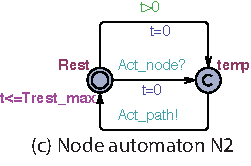
\includegraphics[width=0.3\textwidth]{figs/rule6.pdf}
%	%\vspace{-5pt}
%	\caption{\small Node automata after application of Rule 7}
%	%\vspace{-15pt}
%	\label{fig:rule6}
%\end{figure}

%\subsection{Automatic rule application}
\label{automatedApplication}

Because we start from a set of initial models, and each one may be abstracted using a number of abstraction rules, we have a choice of which rules to apply to which models, and the order in which to apply them.
Depending on which rule is applied when, we end up with different abstract models.
\emph{We seek a rule application order which yields the most abstract model that is still appropriate for the requirement $\phi$}.
In this section we propose a measure of abstractness, and sketch how an optimal order of application can be found as the solution of a Mixed-Integer Nonlinear Program (MINLP).
Due to space limitations the following discussion omits certain details which can be found in the technical report. 

First, we observe that when a rule is applied to a labeled graph $G=(V,E,A)$, it either decreases the number of vertices, or the number of edges, or it enlarges the invariant and/or guard sets of some of the automata (by manipulating the parameters as done, e.g., by rule R4).
Let $\{R_i\}_{i=1}^n$ be the set of abstraction rules, $\{G_s\}_{s=1}^m$ be the initial set of labeled graph heart models, and assume a pre-fixed maximum number of rule applications $N \geq 1$.
We define a measure of the abstraction power $\alpha(R_i,G_s)$ of a rule $R_i$ applied to graph $G_s$ to be
\[\alpha(R_i,G_s) = |V(G_s)| - |V(R_i(G_s))| + |E(G_s)| - |E(R_i(G_s))| + \sum_{x \in \Ec(R_i(G_s))}|\theta^x - R_i(\theta^x)|\] 
Intuitively, a rule $R$ is more abstract than rule $R'$ if it removes more elements or enlarges the parameter ranges more.
Then if we apply rules $R_{i_1}, R_{i_2},\ldots, R_{i_N}$ in that order to the set $\{G_i\}$, the abstractness of the final model is given by given by
$\alpha = \sum_j \alpha(R_{i_j},G_{i_j})$
where $G_{i_j}$ is the graph to which $R_{i_j}$ was applied.

Rule application must respect the following constraints, all of which can be encoded as the constraints of a MINLP:
\begin{enumerate}
	\item Only one rule can be applied at a time.
	\item A rule can only be applied to a (sub)graph with a given structure, and whose parameters respect certain conditions.
	\item When a rule is applied to a subgraph, it may disable future rule applications to this subgraph, either because a) it changed the subgraph's structure, or b) it updated the subgraphs's parameters.
\end{enumerate}
We define binary variables $a_{isj}$ such that $a_{isj} = 1$ iff at the $j^{th}$ time step, we apply rule $R_i$ to graph $G_s$.
The first constraint, for example, can be encoded as
\[\forall j=1,\ldots, N, \sum_{i,s}a_{isj} \leq 1\]

Proceeding in this manner, we formulate a MINLP whose solution gives an optimal order of rule application, in the sense of maximizing $\alpha$.
Then model-checking can be performed on this most abstract model returned by the optimization.





%\section{Model checking with the abstraction tree}
\label{modelCheckingwAbstTree}


	\begin{enumerate}
		\item Measure of abstractness; define 'appropriate for the requirement'
		\item Search procedure
		\item What happens if a counter-example is found
		\item Elaborate example
		\end{enumerate}
\section{Closed-loop Model Checking With Abstraction Tree}
%\subsection{Heart Model Abstraction Tree}
A set of heart models corresponding to different heart conditions are first developed. 
The list can be expanded as new heart conditions are discovered.
Because we start from a set of initial models, and each one may be abstracted using a number of abstraction rules, we have a choice of which rules to apply to which models, and the order in which to apply them.
Depending on which rule is applied when, we end up with different abstract models.
Thus an \emph{abstraction tree} $T_{HM}$ for the heart is created, as shown in \figref{HM_abs}. 
%Note that applying rules in different order results different abstraction tree. 
%The order used to obtain $HM\_tree$ is based on the domain knowledge that certain heart conditions may have similar behaviors and similar inputs to the pacemaker. 
%This systematic grouping maintains the physiological-relevance of the heart model even at higher abstraction levels, and reduce the necessity to resolve ambiguities at lower abstraction levels when model checking certain requirements.
\begin{figure}[!t]
	\centering
	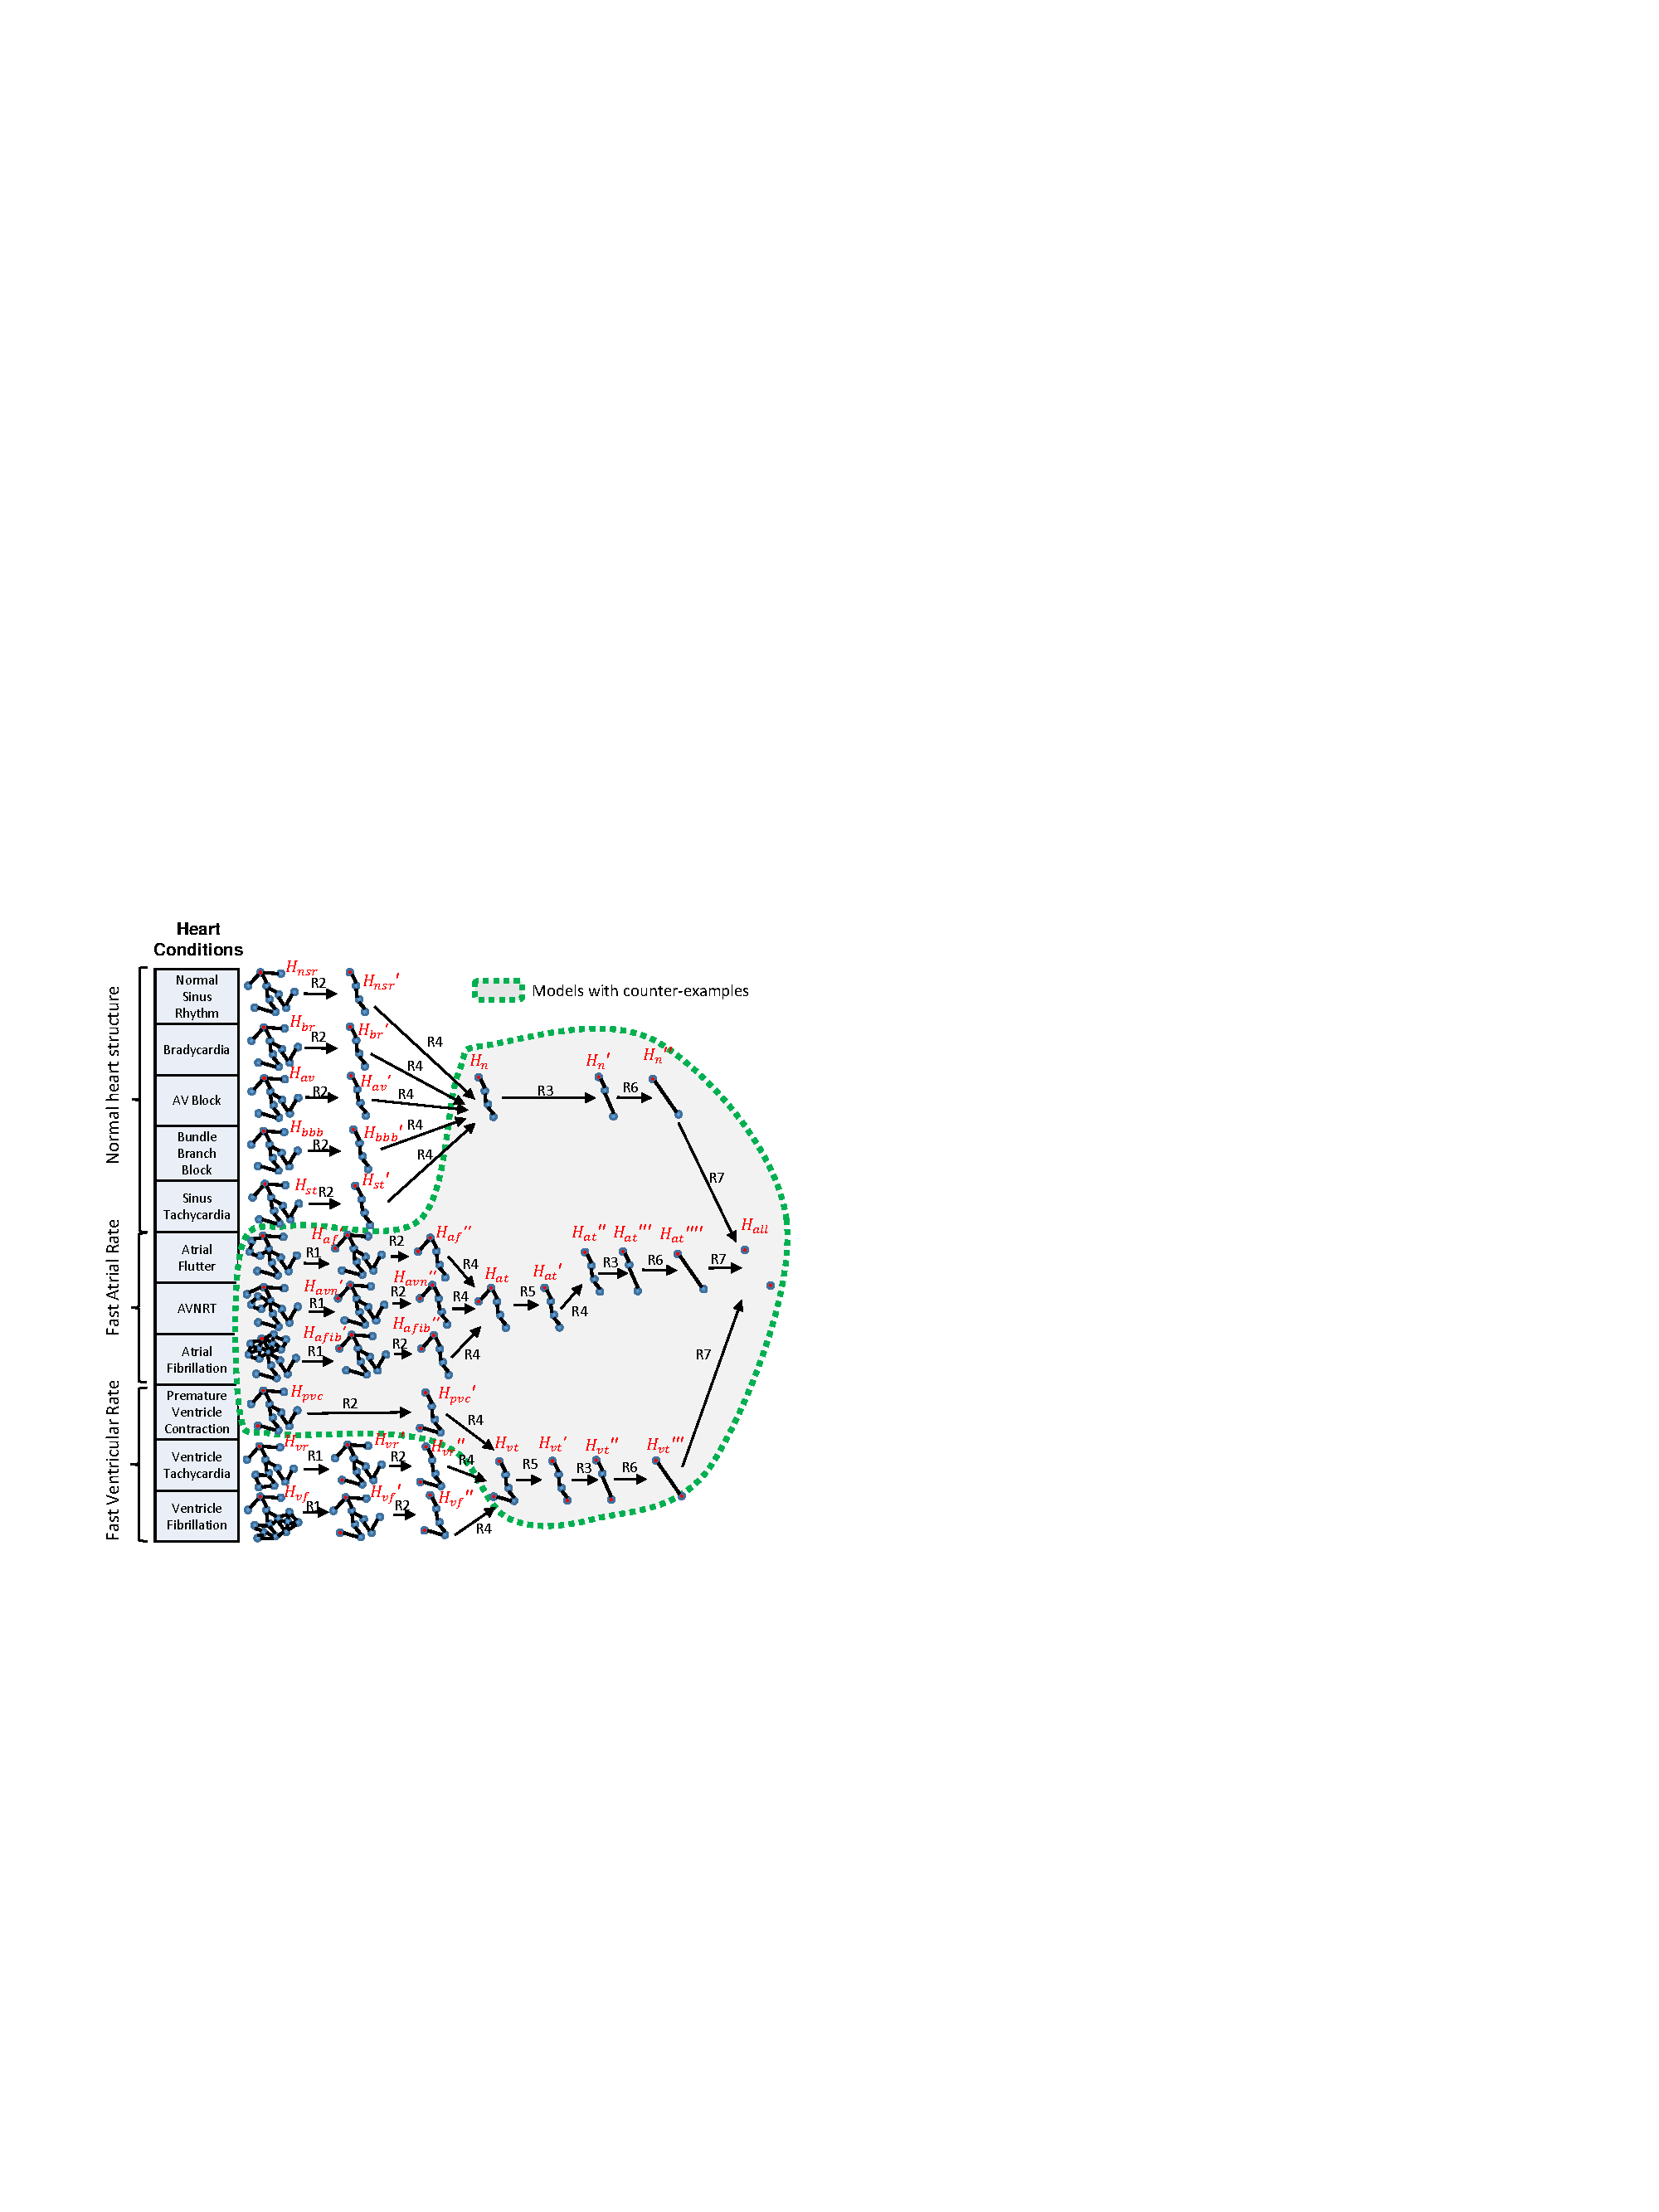
\includegraphics[width=0.85\textwidth]{figs/abs.pdf}
	%\vspace{-5pt}
	\caption{\small Heart Model Abstraction Tree}
	\vspace{-15pt}
	\label{fig:HM_abs}
\end{figure}
%\subsection{Model Checking Procedure}
After the abstraction tree is built, it can be used for closed-loop model checking by non-domain experts. 
The question is which models to select from the abstraction tree to perform model checking, and provide the most concrete counter-examples.
These counter-examples are provided to the physicians, along with the heart models that generated them, to determine their physiological validity.

We now summarize the model checking procedure, and give a detailed example in the next section.
Recall the definition of appropriateness from Section \ref{preliminaries}.

\ifthenelse{\boolean{TECH_REPORT}}{\begin{proof}
	\newcommand{\hs}{\hat{s}}
	To prove that $Var(\varphi) \subset Var(M)$ is a sufficient condition for appropriateness, we introduce some standard terminology.
	For an integer $n \geq 1$, $[n] = \{1,\ldots,n\}$.
	Given a tuple $(a_1,a_2,\ldots,a_n)$ and a subset $H \subset [n]$, the projection function $\proj{}{H}$ retains the components indexed by $H$. E.g., $\proj{(a_1,a_2,a_3)}{1,3} = (a_1,a_3)$.
	
	Let $\Vc = \{V_1,\ldots, V_n\}$ be variables with valuation domains $D_1,\ldots,D_n$, respectively. 
	Let $D = D_1 \times \ldots D_n$ be the state space.
	Let $AP$ be the set of atomic propositions on $\Vc$, i.e. expressions involving the variables in $\Vc$.
	We write $Var(p)$ for the variables that appear in a given proposition $p$, and $Var(\varphi) = \cup_{p \textrm{ in } \varphi} Var(p)$.
	We define the map $\Oc: AP \rightarrow 2^D$ which assigns to each atomic proposition $p$ a subset $\Oc(p)$ of states where the proposition holds.
	Conversely, $\Oc^{-1}(\{s\})$ is the set of atomic propositions that hold for a state $s \in D$.

	Given a proposition $p$, if a variable $v_1$ is not in $Var(p)$, then $\proj{\Oc(p)}{1} = D_1$.
	I.e., $p$ places no constraints on the value of variable $v_1$.
	Given a trace $x = s_0 s_1 s_3 \ldots \in D^\omega$, we define a \emph{run} for $x$ to be the sequence $p_o p_1 p_2 \ldots$ of atomic propositions such that $p_i \in \Oc^{-1}(s_i)$.
	Let $\varphi$ be a formula on $AP$.
	If two traces $x$ and $y$ have the same run and $x \models \varphi$, then $y \models \varphi$.
	
	All our abstraction rules are projections: i.e., associated to each abstraction function $\absfun$ is a set $H \subset [n]$ of indices such that to for every $s = (a_1,a_2,\ldots,a_n) \in D$, $h(s) = \proj{s}{H}$.
	For rule $\absfun_4$, $H = [n]$.
	
	Now let $M$ be a model, 
	$\absfun = \proj{\cdot}{2,\ldots,n}$, and $M' = h(M)$.
	Suppose that $Var(\varphi) \subset Var(M')$.
	Let $x \in \beh(M')$ such that
	\[x = \hs_0 \hs_1 \hs_2 \ldots \models \varphi\] 
	We want to prove that for any $y \in \absfun^{-1}(x)$, $y \models \varphi$.
	First note that $\hs_i \in D_2 \times \ldots \times D_n$.
	Let $p_0 p_1 p_2 \ldots$ be the run corresponding to $x$.
	By definition of run,
	 $\hs_i \in \Oc(p_i) \cap \proj{D}{2,\ldots,n} = \proj{\Oc(p_i)}{2,\ldots,n}$.
	Since $v_1 \notin Var(M')$, then $v_1 \notin Var(p_i)$ for all $p_i$ in $\varphi$.
	Therefore 
	\[\Oc(p_i) = D_1 \times \proj{\Oc(p_i)}{2,\ldots,n}\; \forall i\]
	For any $y \in \absfun^{-1}(x)$, $y = s_0 s_1 s_2 \ldots$ where $s_i = (a_i, \hs_i) \in D$.
	Thus $s_i \in \Oc(p_i)$, which means that $p_0 p_1 \ldots$ is a run of $y$ as well.
	Therefore, $y \models \varphi$.
	
	
	
	
	\end{proof}
	}{In the technical report \cite{regar_tech}, we show that a sufficient condition for a model $M$ to be appropriate for a requirement $\varphi$ with monitor $Mon$ is
$Var(\varphi) \subset Var(M) \cup Var(Mon)$.}

A search algorithm is developed to select the most abstract models from the abstraction tree $T_{HM}$ that are appropriate for a requirement $Req$. 
\ifthenelse{\boolean{TECH_REPORT}}
{
\begin{figure}[!t]
		\centering
		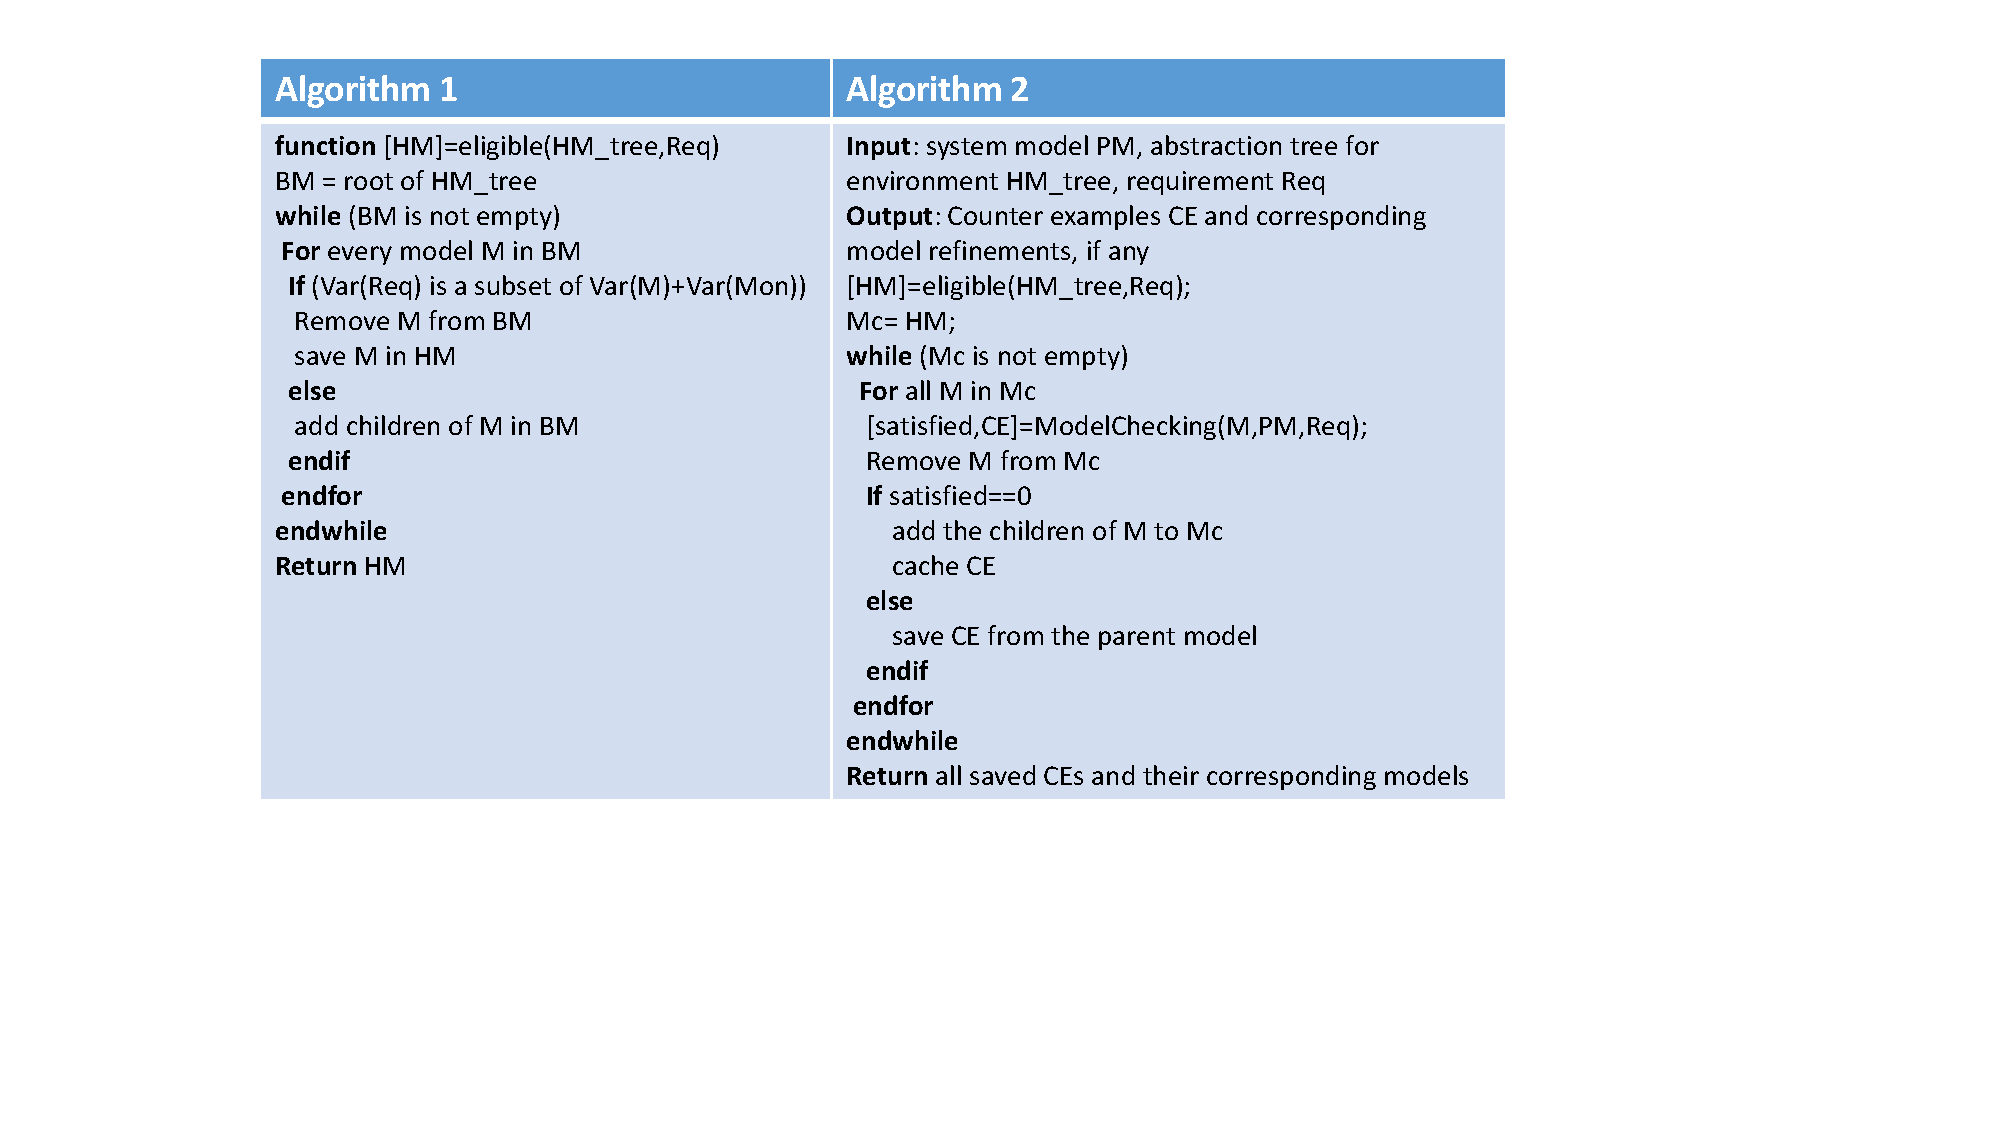
\includegraphics[width=0.9\textwidth]{figs/algorithm.pdf}
		%\vspace{-5pt}
		\caption{\small Algorithms for closed-loop model checking with abstraction tree}
		  \vspace{-10pt}
		\label{fig:algorithm}
\end{figure}}
{The detailed implementation of the algorithm can be found in \cite{regar_tech}.
}

Model checking is run on these models. 
When a run returns a violation, it returns an abstract counter-example $\delta_{cex}$, along with the heart model $M_{cex}$ that generated it.
For each such violation, we search the tree for the most concrete descendant of $M_{cex}$ that still displays a counter-example to $Req$.
This is then provided to the physician along with the counter-example.
%The detailed implementation of the algorithm can be found in \cite{regar_tech}.
%Algorithm 2 (\figref{algorithm}) describes the process for closed-loop model checking with an abstraction tree.


%The most abstract model in the abstraction tree is built to cover the input space to the device as much as possible, thus it may not have enough details to constrain the behaviors of the model according to the constraints in the requirement. Thus the first step of closed-loop model checking is to select the most abstract models which are appropriate for the requirement. A model $M$ is appropriate for a requirement $Req$ if the environment transitions mentioned in the requirement, denoted as $EnvT(Req)$, is a subset of the environment transitions associated with the model $EnvT(M$). The following algorithm finds the most abstract heart models in the abstraction tree $HM\_tree$ that are appropriate for a requirement $Req$.
%\begin{Verbatim}
%Algorithm 1
%function [HM]=eligible(HM_tree,Req)
%BM = root of HM_tree
%while (BM is not empty)
 %For every model M in BM
  %If (Var(Req) is a subset of Var(M)+Var(Mon))
   %Remove M from BM
   %save M in HM
  %else
   %add children of M in BM
  %endif
 %endfor
%endwhile
%Return HM
%\end{Verbatim}
%BM = all models in HM_tree with all Prop(Req)
%For all M in BM
 %while (in the parent of M no behavior in Prop(Req) is abstracted with other behaviors)
	 %M = parent of M
 %endwhile
 %save M in HM
 %endfor

%\begin{Verbatim}
%Algorithm 2
%Input: system model PM, abstraction tree for environment HM_tree, requirement Req
%Output: Counter examples CE and corresponding model refinements, if any
%[HM]=eligible(HM_tree,Req);
%Mc= HM;
 %while (Mc is not empty)
  %For all M in Mc
   %[satisfied,CE]=ModelChecking(M,PM,Req);
	 %Remove M from Mc
	 %If satisfied==0
	  %add the children of M to Mc
		%cache CE
	%else
		%save CE from the parent model
	%endif
 %endfor
%endwhile
%Return all saved CEs and their corresponding models
%\end{Verbatim}

\section{Case Study: Closed-loop Model Checking of a Dual Chamber Pacemaker}
\label{caseStudy}
\begin{figure}[!t]
	\centering
	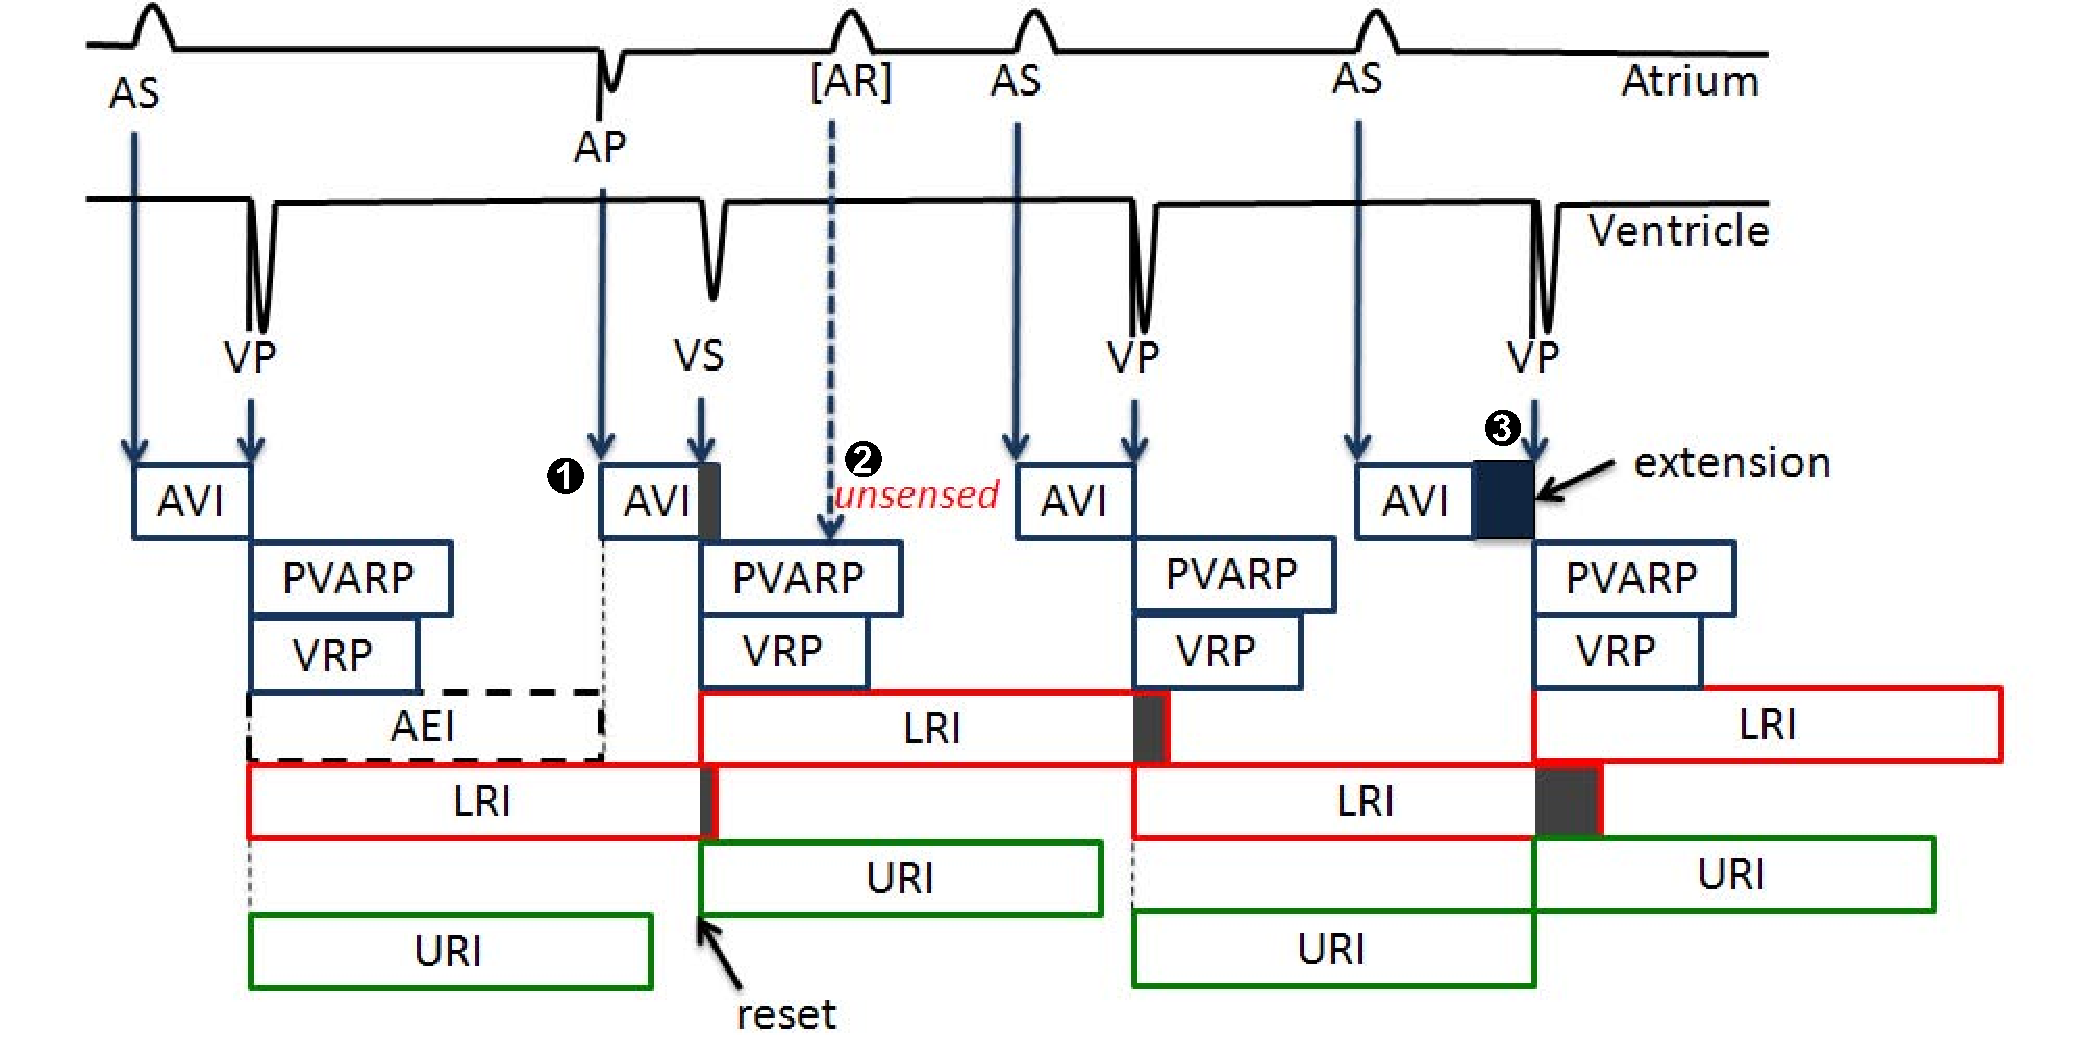
\includegraphics[width=0.8\textwidth]{figs/PM_timers.pdf}
	\vspace{-10pt}
	\caption{\small Basic timers for a dual chamber pacemaker. AS: Atrial Sense, VS: Ventricular Sense, AP: Atrial Pacing, VP: Ventricular Pacing.}
	\vspace{-10pt}
	\label{fig:PM_timers}
\end{figure}

\subsection*{Step 1: The Pacemaker Model}
A pacemaker diagnoses heart conditions and delivers electrical pacing to the heart according to the timing intervals between events from the heart and the pacemaker itself. 
In this section we use a simple dual chamber pacemaker as example for closed-loop model checking. 
The detailed UPPAAL timed automata implementation of the model can be found in \cite{sttt13}. 
A dual chamber pacemaker has several basic timers, which are shown in \figref{PM_timers}:\\
\textbf{Atrial Escape Interval (AEI)} defines the maximum interval between the last ventricular event (VS,VP) to an atrial event (AS,AP). 
If no AS happened before the AEI timer expires, atrial pacing (AP) is delivered to the heart (Marker 1 in \figref{PM_timers}). \\
\textbf{Atrio-Ventricular Interval (AVI)} defines the maximum interval between the most recent atrial event (AS,AP) to a ventricular event (VS,VP). 
If no VS happened before AVI timer expires, and the time since the most recent ventricular event (VS,VP) is no less than URI, ventricular pacing (VP) is delivered to the heart (Marker 3 in \figref{PM_timers}).\\
\textbf{Post-Ventricular Atrial Refractory Period (PVARP) and Ventricular Refractory Period (VRP)} define the minimum period that a AS or VS can happen since the most recent ventricular event (VS,VP). 

%The interactions between the heart and the pacemaker are modeled by using binary event channels. For the atrial lead, we have:
%\textsf{$N_A.Act\_path!\rightarrow$AS!},
%and for ventricular lead we have
%\textsf{$N_V.Act\_path!\rightarrow$VS!}.\\
%The pacemaker accordingly generates atrial or ventricular pacing actions \textsf{AP!$\rightarrow N_A.Act\_node!$} and \textsf{VP!$\rightarrow N_V.Act\_node!$}.
	\vspace{-10pt}
\subsection*{Step 2: Requirement Encoding}
The following requirement is designed to prevent the pacemaker from pacing too fast: 
``If the intervals between self-activations of the atria are between 300ms to 1000ms (60bpm-200bpm), the intervals between ventricular paces should be no shorter than 500ms.''
Self-activation of the atria can be expressed using the location and clock of of node automaton $N_A$.
The requirement can be formalized using the monitor  $M_{sing}(VP,500,\infty)$:
%\hatodo{mention $N_A$ is the atrium node automaton}
\[Req1: N_A.loc=Rest \land N_A.t\in [300,1000] \Rightarrow \neg M_{sing}.loc==Err\]
%\todo[inline]{some figure captions are all caps, others are not. please use same thing throughout}
%\begin{figure}[!b]
	%\centering
	%\vspace{-10pt}
	%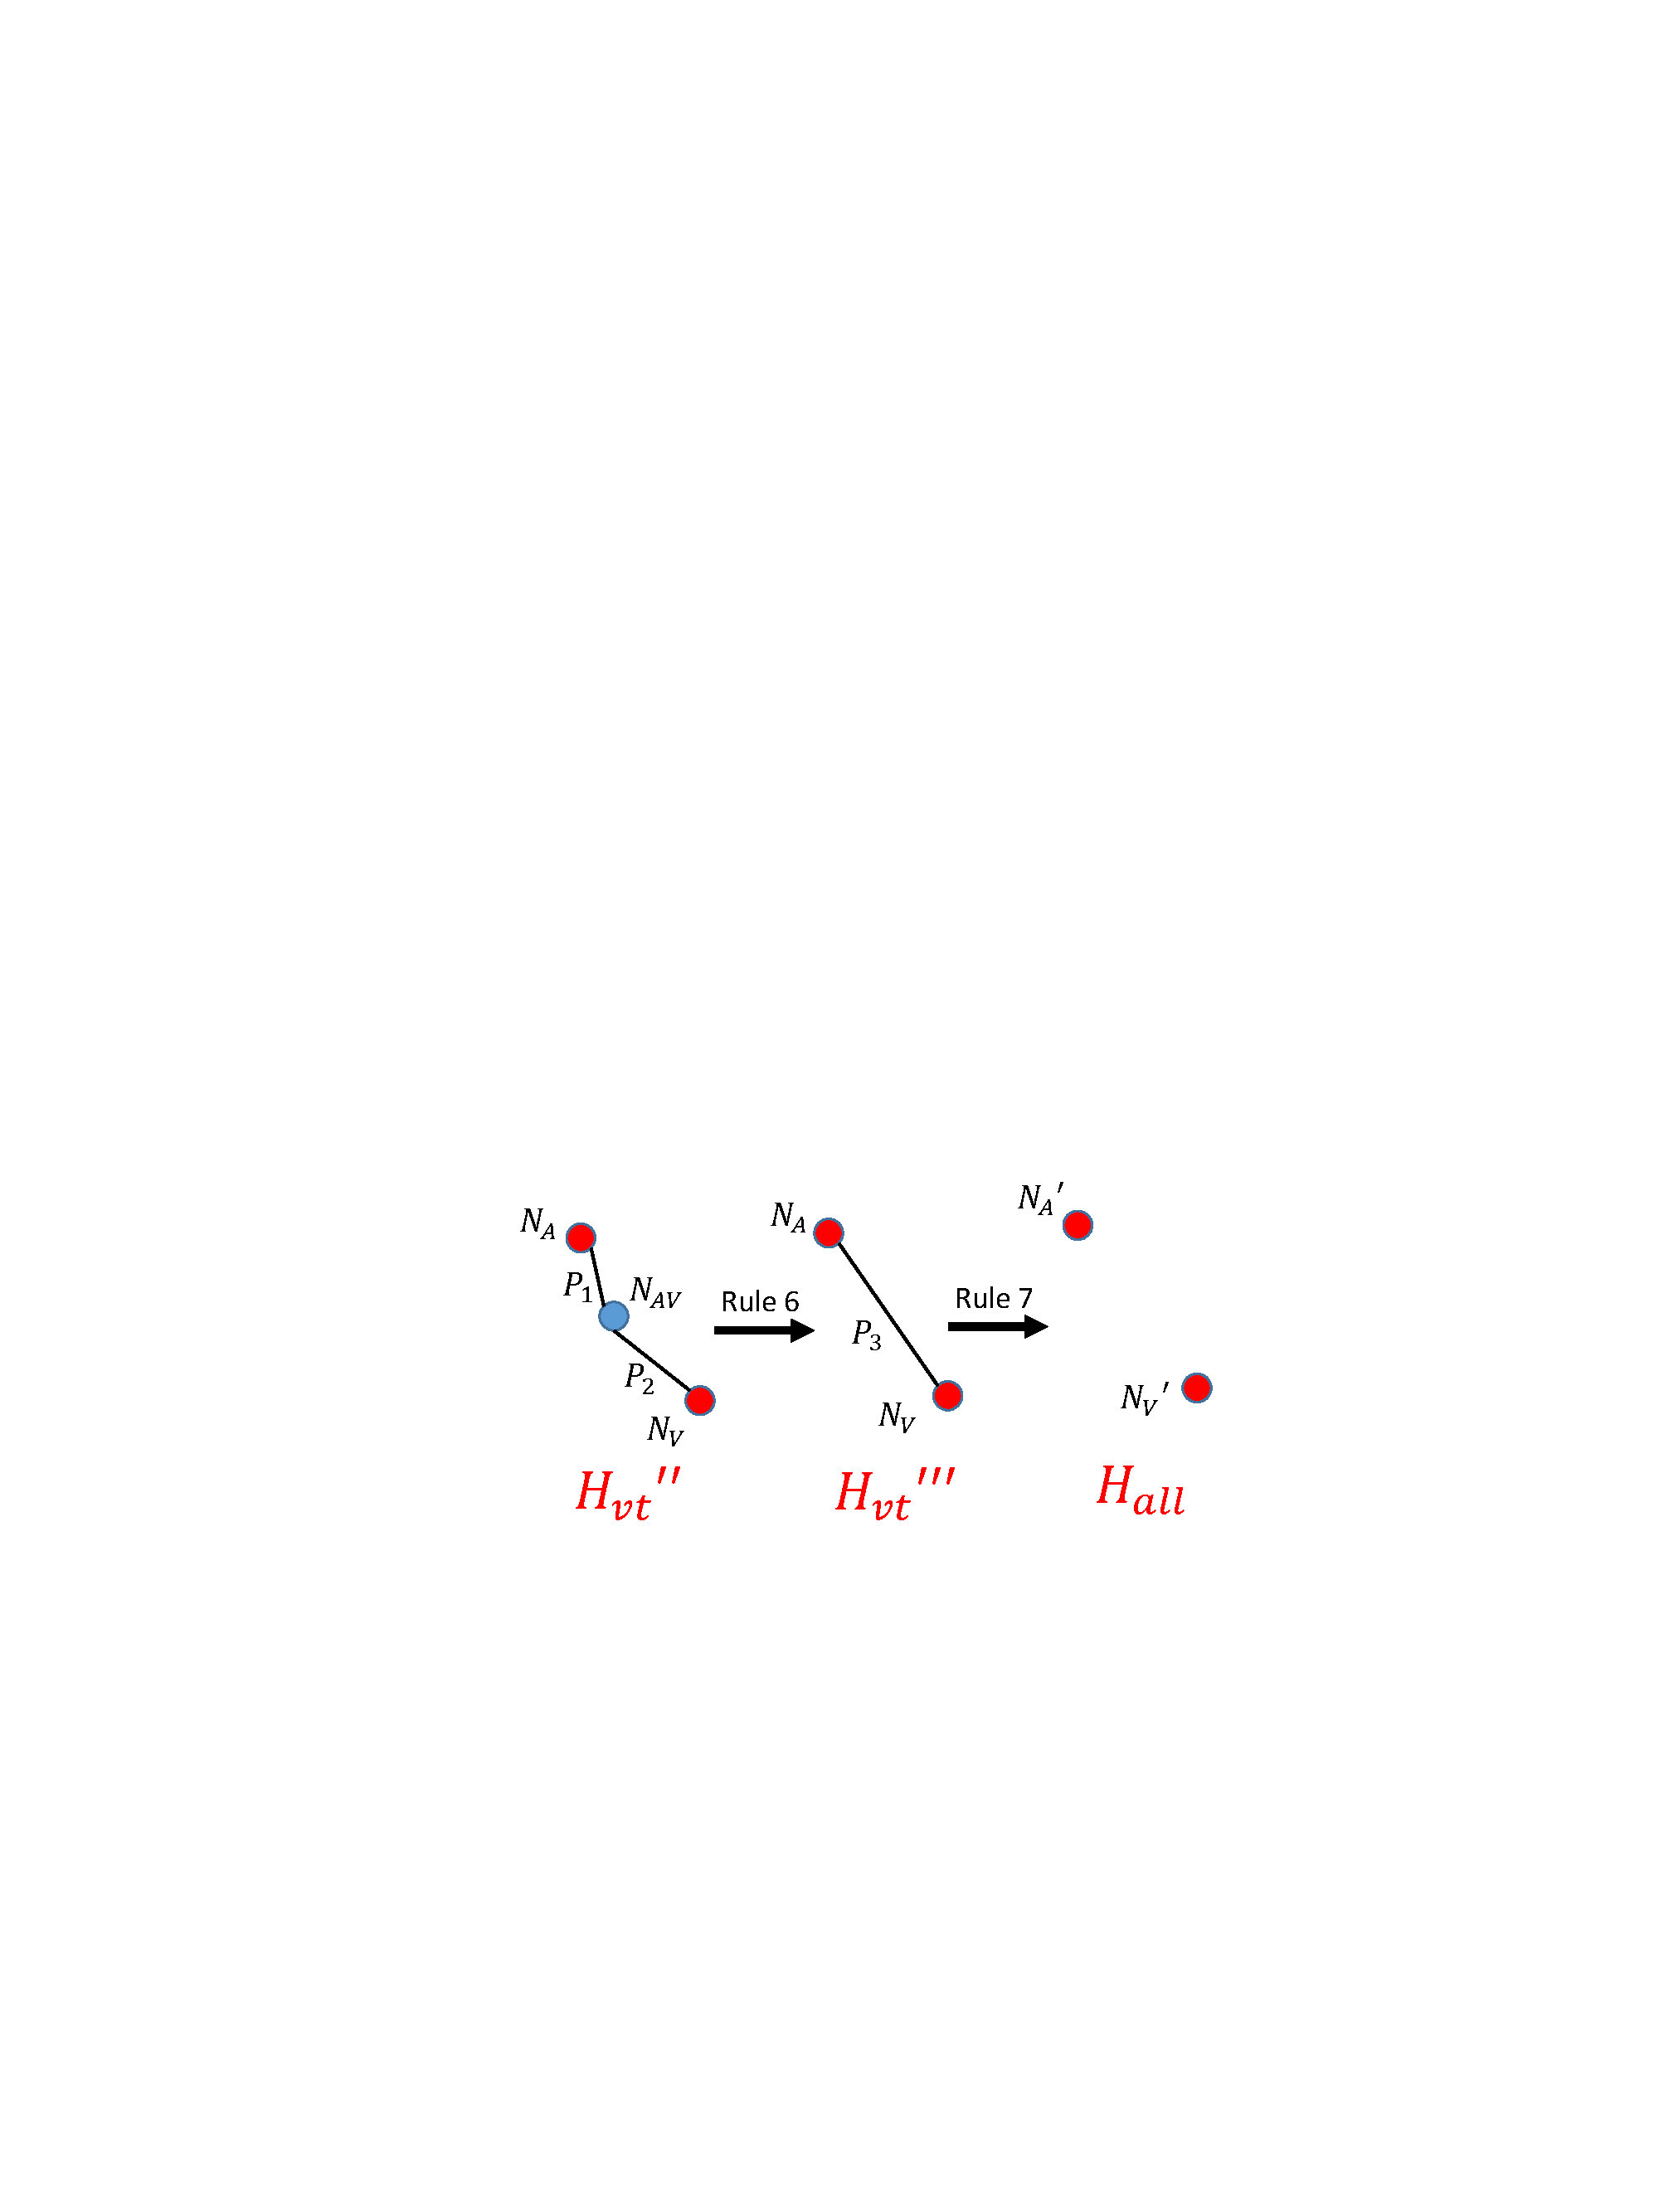
\includegraphics[width=0.5\textwidth]{figs/abs_sim.pdf}
%
	%\caption{\small Abstraction Rule Application Example}
%\vspace{-10pt}
	%\label{fig:abs_exam}
%\end{figure}
 \subsection*{Step 3: Choosing Appropriate Heart Models For the Requirement}
To verify the closed-loop system with pacemaker model $PM$ and abstraction tree $T_{HM}$ (\figref{HM_abs}) against requirement $Req1$, the most abstract appropriate models are selected from the tree. 
The single event monitor $M_{sing}$ from \figref{monitor}.a with variables $Var(M_{sing})=\{M_{sing}.t,M_{sing}.loc\}$ is used for this requirement. 
The variables in the requirement are:
$Var(Req1)=\{N_A.t,N_A.loc,M_{sing}.loc\}$.

At the root of the tree $H_{all}$, we have $\{N_A.t,N_A.loc\} \not \subset Var(H_{all})\cup Var(M_{sing})$. 
So $H_{all}$ is not appropriate for $Req1$. 
All the children of $H_{all}$: $H_n'',H_{at}'''',H_{vt}'''$ are appropriate for $Req1$,
%we have $Var(Req1)\cup Var(M_{sing})\subset Var(H_n'')=Var(H_{at}'''')=Var(H_{vt}''')$, 
thus these 3 heart models are output as the most abstract models that are appropriate for $Req1$.
\begin{figure}[!t]
	\centering
	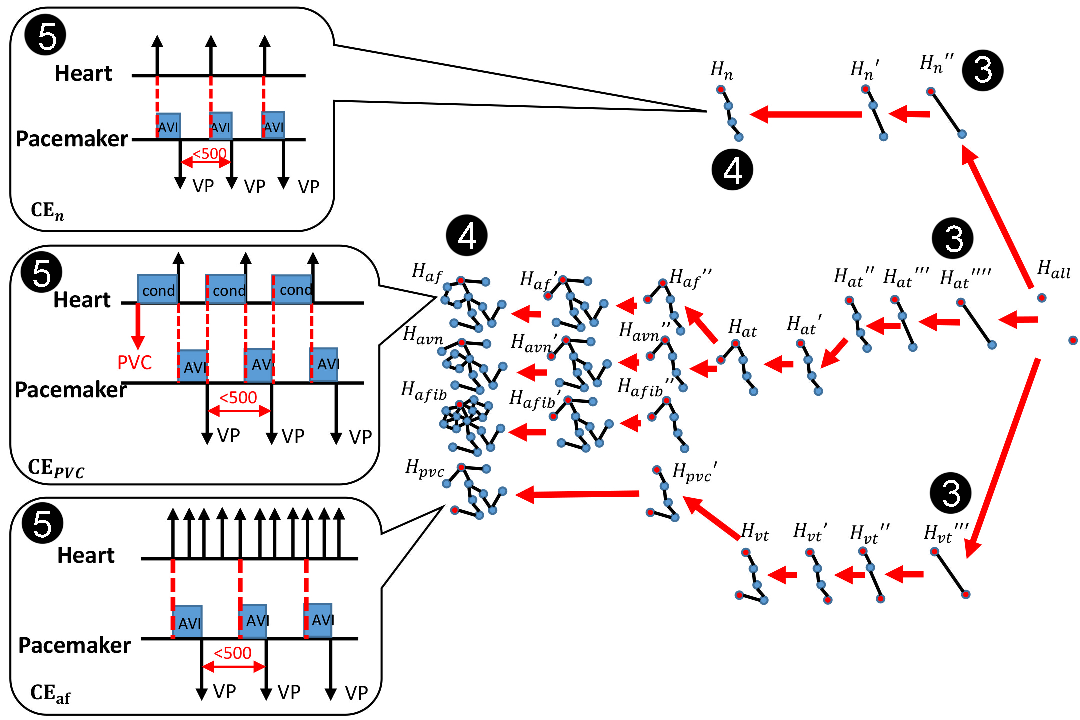
\includegraphics[width=0.8\textwidth]{figs/abs_rev.pdf}
	%\vspace{-5pt}
	\caption{\small Finding the most concrete counter-examples using the abstraction tree}
	\vspace{-10pt}
	\label{fig:CE}
\end{figure}
	\vspace{-10pt}
\subsection*{Step 4: Return the most Concrete Counter-Examples}
After the appropriate models for $Req1$ are selected, we have the initial set
$HM=\{H_n'',H_{at}'''',H_{vt}'''\}$.
Then we run Algorithm 2. By model checking on all 3 initial models in UPPAAL we have: 
$$H_n''||PM\not\models Req1;\; H_{at}''''||PM\not\models Req1;\; H_{vt}'''||PM\not\models Req1$$
%$$[1,[]]=ModelChecking(H_n'',PM,Req1)$$
 %$$[0,CE_1]=ModelChecking(H_{at}'''',PM,Req1)$$
%$$[0,CE_2]=ModelChecking(H_{vt}''',PM,Req1)$$
%\hatodoin{In the following text you use $CE_{at}$, etc. It's  best to use the letter subscripts in the above equations as well, so it's clear which cex comes from which heart model.}
%For the two heart models $H_{at}'''',H_{vt}'''$ in which the requirement is violated, the algorithm keeps going down the abstraction tree, and upon termination counter-examples are returned for the following heart models
The abstraction tree is then further explored. The heart models with counter-examples are illustrated in \figref{HM_abs}, and the most refined heart models with counter-examples are: $H_{n};H_{pvc};H_{af};H_{avn};H_{afib}$.
%$$[0,CE_{at}]=ModelChecking(H_{at},PM,Req1)$$
%$$[0,CE_{pvc}]=ModelChecking(H_{pvc},PM,Req1)$$
%$$[0,CE_{af}]=ModelChecking(H_{af},PM,Req1)$$
%$$[0,CE_{avn}]=ModelChecking(H_{avn},PM,Req1)$$
%$$[0,CE_{afib}]=ModelChecking(H_{afib},PM,Req1)$$

%\begin{figure}[!t]
		%\centering
		%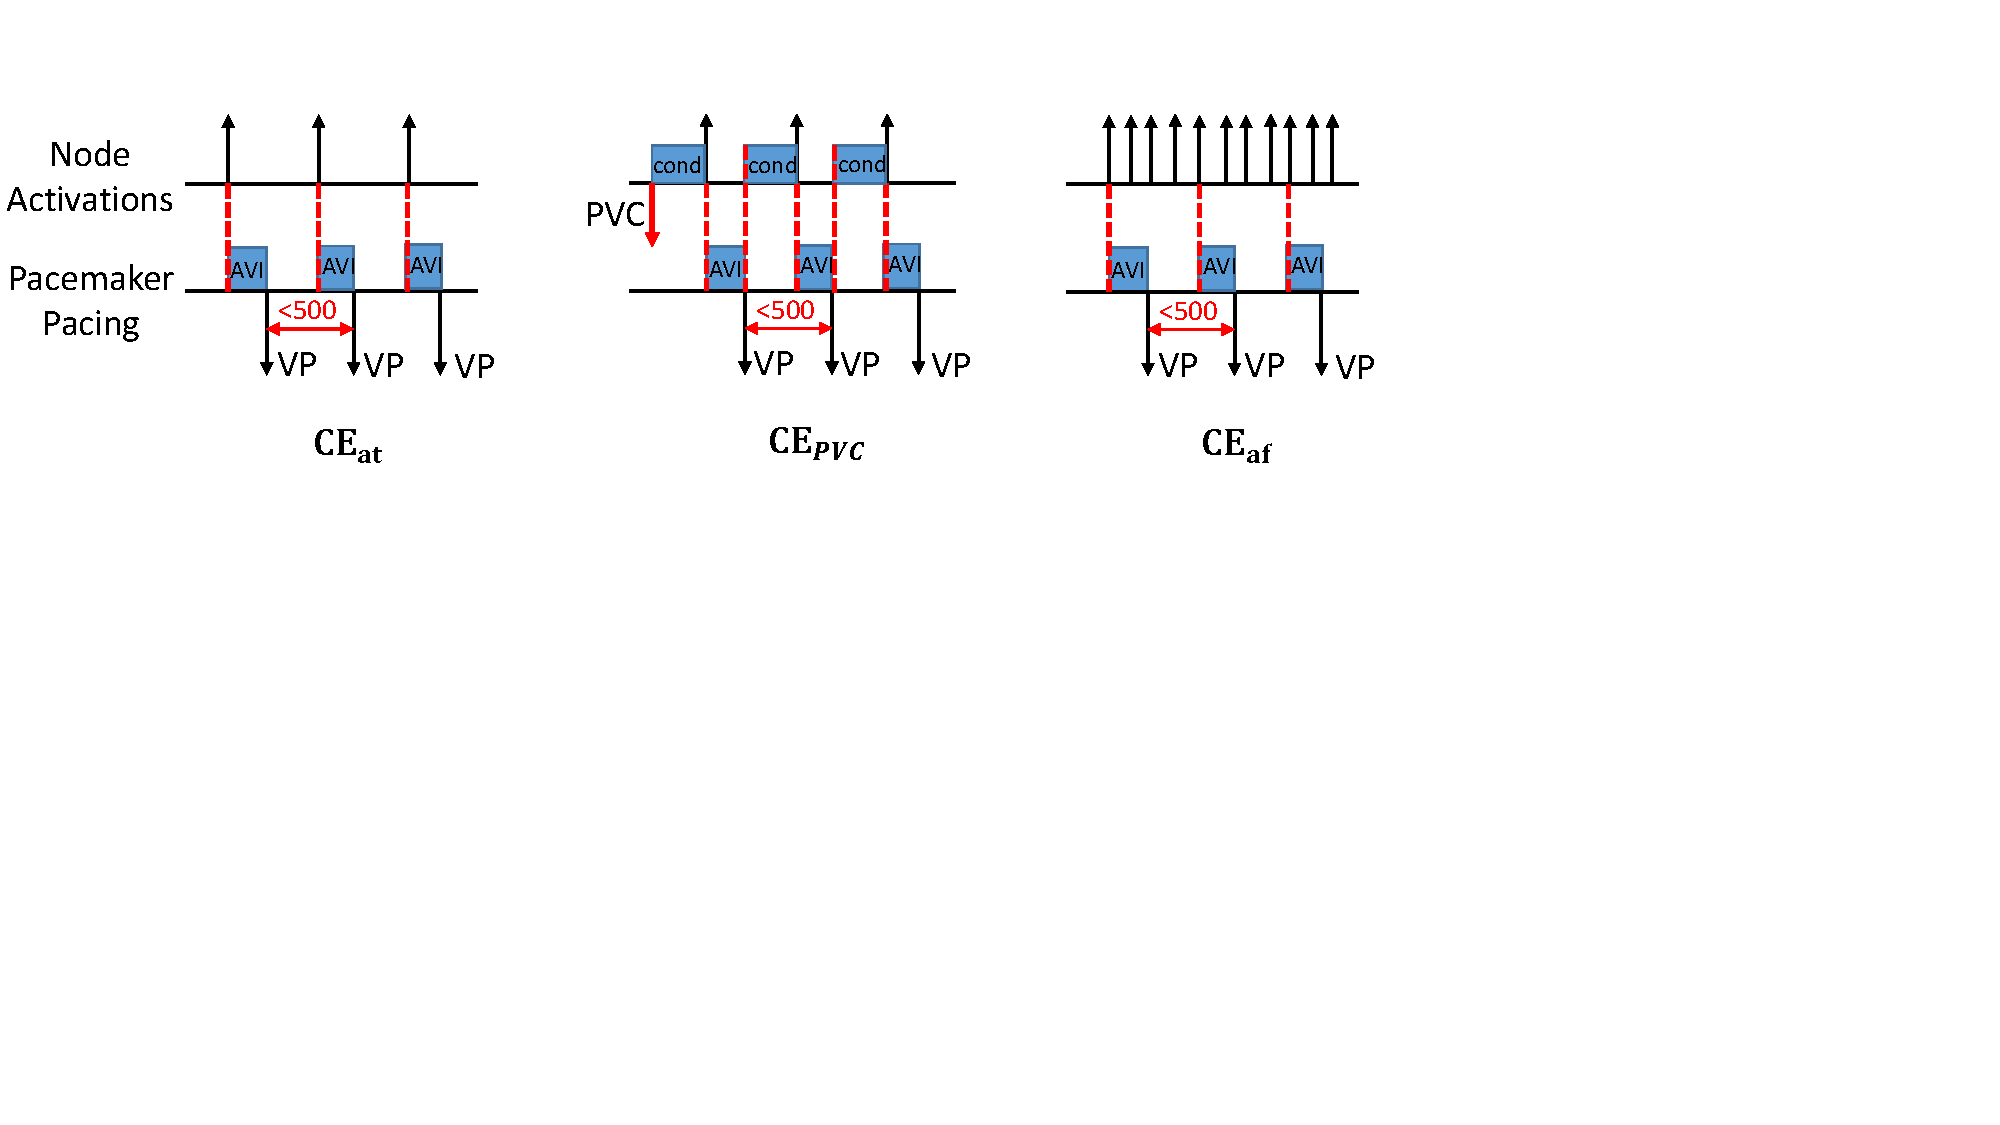
\includegraphics[width=0.9\textwidth]{figs/case.pdf}
		%%\vspace{-5pt}
		%\caption{\small Counter-examples}
		  %\vspace{-10pt}
		%\label{fig:CE}
%\end{figure}
	\vspace{-10pt}
\subsection*{Step 5: Analysis of the Counter-examples}
The counter-examples are then shared with physicians for analysis. In \figref{CE} we demonstrate 3 counter-examples. In the counter-examples, the first signal shows the intrinsic heart signals over time with up arrows as atrial activations and down arrows as ventricular activations. The second signal shows the pacemaker outputs with up arrows as atrial pacing and down arrows as ventricular pacing.%We only show the activations of the atrial node and ventricle pacing. 

$CE_{n}$ is returned by $H_n$ and none of its children models violate the requirement. By careful analysis we found that $CE_{n}$ features the combination of fast intrinsic atrial rate and prolonged A-V conduction delay, which is the combination of heart conditions $H_{st}$ and $H_{av}$. This scenario shows that the abstraction rules can introduce physiological heart conditions that were not explicitly modeled in the initial model set. The pacemaker improved the open-loop heart condition by pacing the ventricles $AVI$ after each atrial event, which is a correct operation of the pacemaker despite the requirement violation. %\hatodo{is it TAVI or AVI like in the previous seciton?}

%\hatodoin{Do you mean that $CE_{at}$ is not a bug? Does this mean that the requirement may be violated in ways that are not dangerous?}
$CE_{pvc}$ has a very similar execution to $CE_{n}$. However, the activations of the atrial node are triggered by retrograde conduction from ventricular paces (marker \textsf{cond}). The atrial activations trigger another ventricular pace after $AVI$, which will trigger another retrograde conduction. In this case the heart rate is inappropriately high, which corresponds to a dangerous closed-loop behavior referred to as \emph{Endless Loop Tachycardia}.

In $CE_{af}$ the atrial rate is very high, which is also a sub-optimal but not dangerous heart condition. 
However, the ventricular rate can stay normal due to the blocking property of the AV node. 
Despite the filters in the pacemaker, the pacemaker still paces the ventricle for every 3 atrial activations, which extends fast atrial rate to more dangerous fast ventricular rate. 
%\hatodoin{Not very clear..do you mean that the intrinsoc centricular rate is fine because of AV filtering, but the PM is accelarating it?}
This scenario is referred to as Atrial Tachycardia Response of a pacemaker. 

From the analysis, pacemaker operations in $CE_{pvc}$ and $CE_{af}$ must be revised. However, the revision should not affect the behavior in $CE_{n}$. This example demonstrates that counter-examples from refined models provide more physiological context of the requirement violations, and distinguish the physiological conditions that can trigger the violations. The information is helpful for debugging and improving the algorithm. The physicians can also improve the physiological requirement so that these heart conditions can be then considered case by case. %Both $CE_b$ and $CE_c$ are inappropriate executions of the pacemaker .$CE_a$ and $CE_b$ can have the same input-output executions on the pacemaker side and can only be differentiated on the heart model side. After the physician examines the counter-example the programmer can work on debugging. 
%$NA\_self$ is in $H_3$, we go one level up, in $H_4$ the behavior is not merged with any other parameters. In $H_5$ $NA\_self$ is merged with  $NA'-NV'.cond$ so $H_4$ is returned as the appropriate heart model for R1. In \cite{STTT13} we used $H_4$ to verify the correctness of the ELT termination algorithm. With a basic DDD pacemaker we have $H_4 || P_{DDD}\models R1$. The counter-example returned is exactly the ELT behavior. Then we implement the ELT termination algorithm and we have  $H_4 || P_{ELT}\not\models R1$, meaning ELT has been successfully terminated, and only the ELT is terminated. 
%
%\subsection{Inappropriate Model Refinements}
%If we follow the traditional CEGAR framework and verify the property using $H_5$, an abstract counter-example would return, which is shown in %\figref{C_amiguity}. However the counter-example correspond
 






\vspace{-10pt}
\section{Conclusion}
\vspace{-10pt}
\label{conclusions}
In this paper we addressed the challenges for environment modeling during closed-loop model checking of medical device software. Physiological abstraction rules can be defined to increase coverage of physiological conditions beyond explicitly modeled conditions. By using the abstraction tree constructed by applying the physiological abstraction rules, closed-loop model checking returns the most concrete counter-examples with physiological context to the physician when a physiological requirement is violated. In this paper we use implantable pacemaker as case study but the framework can extend to other domains.

In the future, application of the abstraction rules will be automated. The application of this framework can also be extended to other Cyber-Physical domains.
\bibliographystyle{abbrv}
\vspace{-15pt}
\bibliography{bibliography}





\end{document}